%% For double-blind review submission, w/o CCS and ACM Reference (max submission space)
%\documentclass[sigconf,review,anonymous]{acmart}\settopmatter{printfolios=true,printccs=false,printacmref=false}
%% For double-blind review submission, w/ CCS and ACM Reference
% \documentclass[sigconf,review,anonymous]{acmart}\settopmatter{printfolios=true}
%% For single-blind review submission, w/o CCS and ACM Reference (max submission space)
\documentclass[sigconf,review]{acmart}\settopmatter{printfolios=true,printccs=false,printacmref=false}
%% For single-blind review submission, w/ CCS and ACM Reference
% \documentclass[sigconf,review]{acmart}\settopmatter{printfolios=true}
%% For final camera-ready submission, w/ required CCS and ACM Reference
% \documentclass[sigconf]{acmart}\settopmatter{}


% !TEX root=../main.tex


%% Basics %%%%%%%%%%%%%%%%%%%%%%%%%%%%%%%%%%%%%%%%%%%%%%%%%%%%%%%%%%%%%%%%%%%%%%

%% Fixes %%

\usepackage{underscore}


%% Fonts %%

\usepackage[utf8]{inputenc}
\usepackage[T1]{fontenc}

\usepackage{stmaryrd}

% \usepackage{tgpagella}
% \usepackage{lucidabr}
\usepackage{libertine}
\usepackage[varqu]{zi4}
\usepackage[libertine]{newtxmath}


%% Programming %%

\usepackage{ifthen}


%% Layout %%

% \usepackage[final]{microtype}


%% Additions %%%%%%%%%%%%%%%%%%%%%%%%%%%%%%%%%%%%%%%%%%%%%%%%%%%%%%%%%%%%%%%%%%%

%% Textual %%

\usepackage{paralist}
\usepackage{quoting}


%% Maths %%

\usepackage{amsmath}
\usepackage{mathpartir}


%% Graphics %%

\usepackage{graphicx}
% \usepackage{xcolor}


%% Tabulations %%

\usepackage{booktabs}
\usepackage{array}


%% Listings %%

% \usepackage[final]{listings}


%% References %%

\usepackage{cleveref}

% !TEX root=../main.tex


%% Fixes %%

\frenchspacing

%% NOTE: uses the same lengths as in `tufte-common.def` and `article.cls`...
\setlength{\bigskipamount}   {3.25ex plus .2ex} %% ...before (sub)section
\setlength{\medskipamount}   {2.3ex  plus .2ex} %% ...after section
\setlength{\smallskipamount} {1.5ex  plus .2ex} %% ...after subsection


%% Numbering %%

% \setcounter{secnumdepth}{2}


%% Compact lists %%
%% NOTE: requires `paralist`

\setlength{\pltopsep}{\smallskipamount}
\setlength{\plpartopsep}{\parskip}
\setlength{\plitemsep}{\parskip}
\setlength{\plparsep}{\parskip}

% !TEX root=../main.tex


%% Helpers %%%%%%%%%%%%%%%%%%%%%%%%%%%%%%%%%%%%%%%%%%%%%%%%%%%%%%%%%%%%%%%%%%%%%

\let\newoperator\DeclareMathOperator


%% Text %%%%%%%%%%%%%%%%%%%%%%%%%%%%%%%%%%%%%%%%%%%%%%%%%%%%%%%%%%%%%%%%%%%%%%%%

\newcommand*{\alert}[1]
  {\textbf{#1}}
\newcommand*{\enquote}[1]
  {``#1''}
\newcommand*{\todo}[1]
  {\ensuremath{\star}\marginnote{\ensuremath{\star}#1}}


%% Lists %%
%% NOTE: requires `paralist`

%% Use compact lists by default
\renewenvironment{itemize}
  {\begin{compactitem}}
  {\end{compactitem}}
\renewenvironment{enumerate}
  {\begin{compactenum}}
  {\end{compactenum}}
\renewenvironment{description}
  {\begin{compactdesc}}
  {\end{compactdesc}}
%% Define starred versions as in-paragraph-lists
\newenvironment{itemize*}
  {\begin{inparitem}}
  {\end{inparitem}}
\newenvironment{enumerate*}
  {\begin{inparenum}}
  {\end{inparenum}}
\newenvironment{description*}
  {\begin{inpardesc}}
  {\end{inpardesc}}


%% Blocks %%

\newenvironment{block}
  {\smallskip}
  {\smallskip}


%% Column types %%
%% NOTE: requires `array`

\newcolumntype{L}{>{$}l<{$}}
\newcolumntype{C}{>{$}c<{$}}
\newcolumntype{R}{>{$}r<{$}}
\newcolumntype{T}{>{\ttfamily}l}
\newcolumntype{S}{>{\sffamily}l}


%% References %%
%% NOTE: requires `cleveref`

\let\see\cref
\let\See\Cref
\let\at\cpageref


%% Citations %%
%% NOTE: requires `natbib`

\let\cite\citep
\let\textcite\citet


%% Math %%%%%%%%%%%%%%%%%%%%%%%%%%%%%%%%%%%%%%%%%%%%%%%%%%%%%%%%%%%%%%%%%%%%%%%%

%% NOTE: change this to \emptyset when using a font that includes a nice standard emptyset
\let\nothing\varnothing


%% Braces %%

\let\<\langle
\let\>\rangle

\newcommand*{\llbrace}
  {\{\!|}
\newcommand*{\rrbrace}
  {|\!\}}


%% Operators %%

\let\lt<
\let\gt>
\let\eq\equiv

\newcommand*{\pp}
  {+\!\!+}


%% Shortcuts %%

\newcommand*{\powerset}
  {\mathcal{P}}

\newcommand*{\NN}{\mathbb{N}}
\newcommand*{\ZZ}{\mathbb{Z}}
\newcommand*{\RR}{\mathbb{R}}
\newcommand*{\CC}{\mathbb{C}}

\newcommand*{\LL}{\mathbb{L}}
\newcommand*{\UU}{\mathbb{U}}
\newcommand*{\BB}{\mathbb{B}}
\renewcommand*{\SS}{\mathbb{S}}

\newoperator{\downto}
  {\;\rightarrow\!\shortmid\;}

\let\to\rightarrow
\let\implies\Rightarrow
\let\infers\vdash

% !TEX root=../main.tex


%% Styles %%%%%%%%%%%%%%%%%%%%%%%%%%%%%%%%%%%%%%%%%%%%%%%%%%%%%%%%%%%%%%%%%%%%%%

\lstdefinestyle{natural}
  {columns=fullflexible
  ,gobble=2
  ,breaklines=true
  ,breakatwhitespace=true
  ,literate=
    %{.}{{$\cdot$}}1
    %{.}{{\ }}1
    {<<}{{$\<$}}1
    {>>}{{$\>$}}1
    {->}{{$\to$\ }}2
    % {--}{{--}}1
    %{_}{{\ }}1
    %{\ "}{{\ \textquotedblleft}}2
    %{"\ }{{\textquotedblright\ }}2
  ,basicstyle={\sffamily}
  ,keywordstyle=[1]{\bfseries}
  ,keywordstyle=[2]{\scshape}
  ,keywordstyle=[3]{}
  %,commentstyle={\itshape}
  %,identifierstyle={\itshape}
  ,emphstyle={\itshape}
  %,stringstyle={\rmfamily}
  ,showstringspaces=false
  ,texcl=true
  ,mathescape=true
  %,escapechar=\$
  %,escapeinside={\{\}}
  ,xleftmargin=1\parindent
  }

\lstdefinestyle{flexible}
  {columns=flexible
  ,gobble=2
  ,fontadjust=true
  ,basicstyle={\ttfamily\small}
  ,commentstyle={\itshape}
  ,keywordstyle={\bfseries}
  %,identifierstyle={\itshape}
  %,stringstyle={\ttfamily}
  ,emphstyle={\itshape}
  ,showstringspaces=false
  ,texcl=true
  ,mathescape=true
  %,escapechar=\$
  %,escapeinside={\{\}}
  ,xleftmargin=1\parindent
  }

\lstdefinestyle{literate}
  {literate=
    {\\}{{$\lambda$}}1
    {\\\$}{{\$}}1 %NOTE: otherwise eaten by `\`, NOTE: prevents \$ to be parsed as math escape
    {\\/}{{$\vee$}}1
    {/\\}{{$\wedge$}}1
    {A.}{{$\forall$}}1
    {E.}{{$\exist$}}1
    {->}{{$\rightarrow$ }}1
    {<-}{{$\leftarrow$}}1
    {<=}{{$\leq$}}1
    {>=}{{$\geq$}}1
    {>>=}{{>>=}}3 %NOTE: otherwise eaten by `>=`
    {\{|}{{$\{\!|\!$}}1
    {|\}}{{$\!|\!\}$}}1
    {\{|*|\}}{{$\{\!|\!\!\star\!\!|\!\}$}}3
  }


%% Definitions %%%%%%%%%%%%%%%%%%%%%%%%%%%%%%%%%%%%%%%%%%%%%%%%%%%%%%%%%%%%%%%%%

%% Tasks %%

\lstdefinelanguage{tasks}
  {sensitive=true
  ,morekeywords=[1]{if,then,else,case,of}
  ,morekeywords=[2]{Bool,Int,String,Store,List}
  ,morestring=[b]"
  ,morecomment=[l]--
  ,morecomment=[n]{\{-}{-\}}
  }[keywords,strings,comments]
\lstdefinestyle{tasks}
  {style=natural
  ,literate=
    {\\}{{$\lambda$}}1
    {>>=}{{$\Then$\ }}1
    {>>?}{{$\Next$\ }}1
    {<&>}{{$\And$\ }}1
    {<|>}{{$\Or$\ }}1
    {<?>}{{$\Xor$\ }}1
    {edit}{{$\Edit$}}1
    {enter}{{$\Enter$}}1
    {store}{{$\Change$}}1
    {fail}{{$\Fail$}}1
    {==}{{$\equiv$\ }}1
    {/=}{{$\nequiv$\ }}1
  }

\lstnewenvironment{TASK}[1][]
  {\lstset{language=tasks,style=tasks,#1}}
  {}
\newmacro{TS}[1][1]
  {\lstinline[language=tasks,style=tasks,#1]}
\newmacro{includeTASK}[2][]
  {\lstinputlisting[language=tasks,style=tasks,#1]{#2}}


%% Flows %%

\lstdefinelanguage{flows}
  {sensitive=true
  ,morekeywords=[1]{module,where,define,using,as,yielding,share,holding,with,do,for,fork,then,when,next,done,on,and,or,not,readonly,writeonly,readwrite}
  ,morekeywords=[2]{Bool,Int,String,Shared,List, Date,Document,Photo, Citizen,Company,Declaration}
  ,morekeywords=[3]{True,False,Just,Nothing,List}
  ,morestring=[b]"
  ,morecomment=[l]--
  ,morecomment=[n]{\{-}{-\}}
  }[keywords,strings,comments]

% \lstMakeShortInline[language=flows,style=natural] | % |
\lstnewenvironment{FLOW}[1][]
  {\lstset{language=flows,style=natural,#1}}
  {}
\newmacro{FL}[1][1]
  {\lstinline[language=flows,style=natural,#1]}
\newmacro{includeFLOW}[2][]
  {\lstinputlisting[language=flows,style=natural,#1]{#2}}


%% Clean %%

\lstdefinelanguage{clean}
  {sensitive=true
  %,alsoletter={ABCDEFGHIJKLMNOPQRSTUVWXYZabcdefghijklmnopqrstuvwxyz_`}
  %,alsoletter={~!@\#$\%^\&*-+=?<>:|\\} %$
  ,morekeywords={from,definition,implementation,import,module,system,code,inline,if,case,of,let,let!,in,where,with,class,instance,generic,derive,dynamic,infix,infixl,infixr}
  ,morestring=[b]"
  ,morestring=[b]'
  ,morecomment=[l]//
  ,morecomment=[n]{/*}{*/}
  }[keywords,strings,comments]

\lstnewenvironment{CLEAN}[1][]
  {\lstset{language=clean,style=flexible,#1}}
  {}
\newmacro{CL}[1][1]
  {\lstinline[language=clean,style=flexible,#1]}
\newmacro{includeCLEAN}[2][1]
  {\lstinputlisting[language=clean,style=flexible,#1]{#2}}


\newlogo[ITASKS]{iTasks}
\newlogo{BPMN}
\newlogo{BPEL}
\newlogo{UML}
\newlogo{WFN}

\newlogo{EDSL}
\newlogo{GUI}

\newlogo{STW}
\newlogo{NWO}

% !TEX root=../main.tex



%% Host language %%%%%%%%%%%%%%%%%%%%%%%%%%%%%%%%%%%%%%%%%%%%%%%%%%%%%%%%%%%%%%%


\newkeyword[IF]  {if}
\newkeyword[THEN]{then}
\newkeyword[ELSE]{else}

\newkeyword[Let]{let}
\newkeyword[In]{in}

\newkeyword[Ref] {ref}


\newmacro{If}[3]
  {\IF #1 \THEN #2 \ELSE #3}



%% Values %%


\newmathcommand{unit}{\<\>}


\newvalue{True}
\newvalue{False}
\newvalue[Not]{not}


\newmacro{str}[1]
  {\text{``#1''}}

\newoperator{Length}{\mathrm{length}}


\newvalue[Map]{map}
\newvalue[Fst]{fst}
\newvalue[Snd]{snd}
\newvalue[Assoc]{assoc}



%% Types %%


\newtype{Unit}
\newtype{Bool}
\newtype{Nat}
\newtype{Int}
\newtype{String}
\newtype[Reference]{Ref}
\newtype{Task}
\newtype{Maybe}

\newtype{Euro}



%% Object language %%%%%%%%%%%%%%%%%%%%%%%%%%%%%%%%%%%%%%%%%%%%%%%%%%%%%%%%%%%%%


\let\And\relax
\newoperator{Then}  {\blacktriangleright}
\newoperator{Next}  {\vartriangleright}
\newoperator{And}   {\Join}
\newoperator{Or}    {\blacklozenge}
\newoperator{Xor}   {\lozenge}
\newoperator{Edit}  {\square}
\newoperator{View}  {\overline{\square}}
\newoperator{Enter} {\boxtimes}
\newoperator{Update}{\blacksquare}
\newoperator{Watch} {\overline{\blacksquare}}
\newoperator{Fail}  {\lightning}

\newoperator{AndOr} {\DEPRECATED}



%% Events %%


\newvalue[Left]   {L}
\newvalue[Right]  {R}


\newvalue[Clear]   {C}
\newvalue[Continue]{N}
\newvalue[Pick]    {P}


\newvalue[First]  {F}
\newvalue[Second] {S}
\newvalue[Here]   {H}



%% Semantic functions %%%%%%%%%%%%%%%%%%%%%%%%%%%%%%%%%%%%%%%%%%%%%%%%%%%%%%%%%%


\newmathcommand{evaluate}[rel]
  {\;\downarrow\;}
\newmathcommand{normalise}[rel]
  % {\;\rightarrow\!\shortmid\;}
  {\;\Downarrow\;}
\newmacro{handle}[1]
  {\mathrel{\;\xrightarrow{\;#1\;}\;}}
\newmacro{drive}[1]
  {\mathrel{\;\xRightarrow{\;#1\;}\;}}


\newmathcommand{Value}[cal]
  {V}
\newmathcommand{Firsts}[cal]
  {F}
\newmathcommand{Interface}[cal]
  {U}
\newmathcommand{Succeeding}[cal]
  {S}



%% Depricated %%%%%%%%%%%%%%%%%%%%%%%%%%%%%%%%%%%%%%%%%%%%%%%%%%%%%%%%%%%%%%%%%%

\newvalue[Execute] {<depricated>}

% !TEX root=pldi2019.tex


%% Helpers %%%%%%%%%%%%%%%%%%%%%%%%%%%%%%%%%%%%%%%%%%%%%%%%%%%%%%%%%%%%%%%%%%%%%

\newmacro{newrule}[4][2]
  {\newmacro{#1}{\inferrule*[lab={#1},right={$#2$}]
    {#3}
    {#4}}}
\newmacro{userule}
  {\usemacro}
\newmacro{refrule}[1]
  {\ifthenelse{\isundefined{#1}}
    {\GenericError{}{Rule `#1` is not defined}{}{}}
    {\textsc{#1}}}


\newif\ifstateful
\statefulfalse
\newmacro{st}[2][1]
  {\ifthenelse{\isempty{#1}}
    {\ifstateful{,\:s#2}\else{}\fi}
    {\ifstateful{,\:[#1]s#2}\else{}\fi}}
\newmacro{St}[1]
  {\ifstateful{,\:\Sigma#1}\else{}\fi}



%% Typing %%%%%%%%%%%%%%%%%%%%%%%%%%%%%%%%%%%%%%%%%%%%%%%%%%%%%%%%%%%%%%%%%%%%%%


\newmacro{RelationT}
  {\Gamma,\Sigma \infers e : \tau}


\newrule{T-Var}
  {x:\tau\in\Gamma}
  {\Gamma,\Sigma\infers x:\tau}


\newrule{T-Abs}
  {\Gamma[x:\tau_1] ,\Sigma \infers e:\tau_2}
  {\Gamma,\Sigma \infers \lambda x : \tau_1 . e :\tau_1 \to \tau_2}

\newrule{T-App}
  {\Gamma,\Sigma \infers e_1:\tau_1\to\tau_2\\
   \Gamma,\Sigma \infers e_2:\tau_1}
  {\Gamma,\Sigma \infers e_1 e_2 :\tau_2}


\newrule{T-If}
  {\Gamma,\Sigma \infers e_1:\Bool\\
   \Gamma,\Sigma \infers e_2:\tau\\
   \Gamma,\Sigma \infers e_3:\tau}
  {\Gamma,\Sigma \infers \If{e_1}{e_2}{e_3}:\tau}


\newrule{T-Pair}
    {\Gamma,\Sigma \infers e_1 : \tau_1 \\
     \Gamma,\Sigma \infers e_2 : \tau_2}
    {\Gamma,\Sigma \infers \tuple{e_1, e_2} :\tau_1 \times \tau_2}


\newrule{T-Ref}
  {\Gamma,\Sigma \infers e:\tau}
  {\Gamma,\Sigma \infers \Ref e :\Reference \tau}

\newrule{T-Deref}
  {\Gamma,\Sigma \infers e:\Reference \tau}
  {\Gamma,\Sigma\infers\ !e:\tau}

\newrule{T-Assign}
  {\Gamma,\Sigma\infers e_1:\Reference \tau\\
   \Gamma,\Sigma\infers e_2:\tau}
  {\Gamma,\Sigma\infers e_1 := e_2:\Unit}

\newrule{T-Loc}
  {\Sigma(l) = \tau}
  {\Gamma,\Sigma\infers l:\Reference \tau}


\newrule{T-Edit}
  {\Gamma,\Sigma \infers e : \tau}
  {\Gamma,\Sigma \infers \Edit e : \Task \tau}

\newrule{T-Fill}
  {\ }
  {\Gamma,\Sigma \infers \Enter \tau : \Task \tau}

\newrule{T-Update}
  {\Gamma,\Sigma \infers e : \Reference \tau}
  {\Gamma,\Sigma \infers \Update e : \Task \tau}


\newrule{T-Fail}
  {\ }
  {\Gamma,\Sigma \infers \Fail : \Task \tau}


\newrule{T-Then}
  {\Gamma,\Sigma \infers e_1 : \Task \tau_1 \\
   \Gamma,\Sigma \infers e_2 : \tau_1 \to \Task \tau_2}
  {\Gamma,\Sigma \infers e_1 \Then e_2 : \Task \tau_2}


\newrule{T-Next}
  {\Gamma,\Sigma \infers e_1 : \Task \tau_1 \\
   \Gamma,\Sigma \infers e_2 : \tau_1 \to \Task \tau_2}
  {\Gamma,\Sigma \infers e_1 \Next e_2 : \Task \tau_2}


\newrule{T-And}
  {\Gamma,\Sigma \infers e_1 : \Task \tau_1 \\
   \Gamma,\Sigma \infers e_2 : \Task \tau_2}
  {\Gamma,\Sigma \infers e_1 \And e_2 : \Task\,(\tau_1 \times \tau_2)}


\newrule{T-Or}
  {\Gamma,\Sigma \infers e_1 : \Task \tau \\
   \Gamma,\Sigma \infers e_2 : \Task \tau }
  {\Gamma,\Sigma \infers e_1 \Or e_2 : \Task \tau}


\newrule{T-Xor}
  {\Gamma,\Sigma \infers e_1 : \Task \tau \\
   \Gamma,\Sigma \infers e_2 : \Task \tau }
  {\Gamma,\Sigma \infers e_1 \Xor e_2 : \Task \tau}


\newrule{T-Appoint}
  {\Gamma,\Sigma\infers e:\Task\tau}
  {\Gamma,\Sigma\infers u \At e:\Task\tau}



%% Evaluation %%%%%%%%%%%%%%%%%%%%%%%%%%%%%%%%%%%%%%%%%%%%%%%%%%%%%%%%%%%%%%%%%%


\newmacro{RelationE}
  {e,s \evaluate v,s'}


\newrule{E-Value}[v\in\set{\lambda x:\tau.e, \unit, l, B, I, S}]
  {\ }
  {v,s\evaluate v,s}

\newrule{E-App}
  {e_1,s\evaluate \lambda x:\tau.e_1',s'\\
   e_2,s'\evaluate v_2,s''\\
   e_1'[x\mapsto v_2],s''\evaluate v_1,s'''}
  {e_1 e_2,s \evaluate v_1,s'''}


\newrule{E-IfTrue}
    {e_1,s\evaluate \True,s'\\
     e_2,s'\evaluate v,s''}
    {\If{e_1}{e_2}{e_3},s\evaluate v,s''}

\newrule{E-IfFalse}
  {e_1,s\evaluate \False,s'\\
   e_3,s'\evaluate v,s''}
  {\If{e_1}{e_2}{e_3},s\evaluate v,s''}


\newrule{E-Pair}
  {e_1,s\evaluate v_1,s'\\
   e_2,s'\evaluate v_2,s''}
  {\tuple{e_1,e_2},s\evaluate\tuple{v_1,v_2},s''}


\newrule{E-Ref}
  {e,s\evaluate v,s'\\
   l\not\in Dom(s)}
  {\Ref e,s\evaluate l,s'[l\mapsto v]}

\newrule{E-Deref}
  {e,s\evaluate l,s'}
  {!e,s\evaluate s'(l),s'}

\newrule{E-Assign}
  {e_1,s\evaluate l,s'\\
   e_2,s'\evaluate v_2,s''}
  {e_1:=e_2,s\evaluate \unit,s''[l\mapsto v_2]}


\newrule{E-Sequence}
  {?}
  {e_1;e_2 \evaluate ?}

\newrule{E-Edit}
  {e,s \evaluate v,s'}
  {\Edit e , s\evaluate \Edit v,s'}

\newrule{E-Fill}
  {\ }
  {\Enter \tau,s \evaluate \Enter \tau,s}

\newrule{E-Update}
  {e,s\evaluate l,s'}
  {\Update e ,s\evaluate \Update l,s'}


\newrule{E-Fail}
  {\ }
  {\Fail,s \evaluate \Fail,s}


\newrule{E-Then}
  {e_1 ,s\evaluate t_1,s'}
  {e_1 \Then e_2,s \evaluate t_1 \Then e_2,s'}

\newrule{E-Next}
  {e_1 ,s\evaluate t_1,s'}
  {e_1 \Next e_2 ,s\evaluate t_1 \Next e_2,s'}


\newrule{E-And}
  {e_1 ,s\evaluate t_1 ,s'\\
   e_2 ,s'\evaluate t_2,s''}
  {e_1 \And e_2 ,s\evaluate t_1 \And t_2,s''}


\newrule{E-Or}
  {e_1 ,s\evaluate t_1 ,s'\\
   e_2 ,s'\evaluate t_2,s''}
  {e_1 \Or e_2 ,s\evaluate t_1 \Or t_2,s''}

\newrule{E-Xor}
  {\ }
  {e_1 \Xor e_2 ,s\evaluate e_1 \Xor e_2,s}


\newrule{E-Appoint}
    {e,s\evaluate t,s'}
    {u \At e,s\evaluate u \At t,s'}



%% Normalisation %%%%%%%%%%%%%%%%%%%%%%%%%%%%%%%%%%%%%%%%%%%%%%%%%%%%%%%%%%%%%%%


\newmacro{RelationS}
  {t,s \stride t',s'}


\newrule{S-Edit}
  { }
  {\Edit v,s \stride \Edit v,s}

\newrule{S-Fill}
  { }
  {\Enter \tau,s \stride \Enter \tau,s}

\newrule{S-Update}
  { }
  {\Update l,s \stride \Update l,s}


\newrule{S-Fail}
  { }
  {\Fail,s \stride \Fail,s}


\newrule{S-ThenStay}[\Value(t_1',s') = \bot]
  {t_1,s \stride t_1',s'}
  {t_1 \Then e_2,s \stride t_1' \Then e_2,s'}

\newrule{S-ThenFail}[\Value(t_1',s') = v_1 \land \Failing(t_2,s'')]
  {t_1,s \stride t_1',s' \\
   e_2\ v_1,s' \evaluate t_2,s''}
  {t_1 \Then e_2,s \stride t_1' \Then e_2,s'}

\newrule{S-ThenCont}[\Value(t_1',s') = v_1 \land \lnot\Failing(t_2,s'')]
  {t_1,s \stride t_1',s' \\
   e_2\ v_1,s' \evaluate t_2 ,s'' \\
   t_2,s'' \stride t_2',s'''}
  {t_1 \Then e_2,s \stride t_2',s'''}

\newrule{S-Next}
  {t_1,s \stride t_1',s'}
  {t_1 \Next e_2,s \stride t_1' \Next e_2,s'}


\newrule{S-And}
  {t_1,s  \stride t_1',s' \\
   t_2,s' \stride t_2',s''}
  {t_1 \And t_2,s \stride t_1' \And t_2',s''}


\newrule{S-OrLeft}[\Value(t_1',s') = v_1]
  {t_1,s  \stride t_1',s'}
  {t_1 \Or t_2,s \stride t_1',s'}

\newrule{S-OrRight}[\Value(t_1',s') = \bot \land \Value(t_2',s'') = v_2]
  {t_1,s  \stride t_1',s' \\
   t_2,s' \stride t_2',s''}
  {t_1 \Or t_2,s \stride t_2',s''}

\newrule{S-OrNone}[\Value(t_1',s') = \bot \land \Value(t_2',s'') = \bot]
  {t_1,s  \stride t_1',s' \\
   t_2,s' \stride t_2',s''}
  {t_1 \Or t_2,s \stride t_1' \Or t_2',s''}


\newrule{S-Xor}
  { }
  {e_1 \Xor e_2,s \stride e_1 \Xor e_2,s}

\newrule{S-Eval}[e \neq e']
    {e,s \evaluate e',s' \\
     e',s' \stride e'',s''}
    {e,s \stride e'',s''}


\newrule{S-Appoint}
  {t,s\stride t',s'}
  {u \At t,s\stride u \At t',s'}


% \newrule{S-Next}[t_1' = \Edit v]
%   {t_1,\Sigma \stride t_1'\st{'}   \\
%    e\ v \evaluate t_2       \\
%    t_2\st{'} \stride t_2'\st{''} }
%   {t_1 \Next e,\Sigma \stride t_2'\st{''}}

% \newrule{S-NextEval}
%   {e_1,\Sigma \stride u_1\st{'}}
%   {e_1 \Next e_2,\Sigma \stride u_1 \Next e_2\st{'}}




%% Normalisation %%


\newmacro{RelationN}
  {e,s \normalise t,s'}


\newrule{N-Done}[\Dirty(s,s'') \cap \Watching(t') = \nothing]
    {e,s \evaluate t,s' \\
     t,s' \stride t',s''}
    {t,s \normalise t',s''}


\newrule{N-Stride}[\Dirty(s,s'') \cap \Watching(t') \neq \nothing]
    {e,s \evaluate t,s' \\
     t,s' \stride t',s'' \\
     t',s'' \normalise t'',s'''}
    {e,s \normalise t'',s''}



%% Handling %%


\newmacro{RelationH}
  {t,s \handle{i} t',s'}

\newrule{H-Change}[v, v' : \tau]
  { }
  {\Edit v,s \handle{v'} \Edit v',s}

\newrule{H-Empty}[v : \tau]
  { }
  {\Edit v,s \handle{\Empty} \Enter \tau,s}

\newrule{H-Fill}[v' : \tau]
  { }
  {\Enter \tau,s \handle{v'} \Edit v',s}

\newrule{H-Update}[s(l), v' : \tau]
  { }
  {\Update l,s \handle{v'} \Update l,s[l \mapsto v']{}}


\newrule{H-PassThen}
  {t_1,s \handle{i} t_1',s'}
  {t_1 \Then e_2,s \handle{i} t_1' \Then e_2,s'}

\newrule{H-PassNext}
  {t_1,s \handle{i} t_1',s'}
  {t_1 \Next e_2,s \handle{i \neq \Continue} t_1' \Next e_2,s'}

\newrule{H-Next}[\Value{(t_1,s)}\equiv v_1 \wedge \neg\Failing{(t_2,s')}]
  {e_2 v_1,s\stride t_2,s'}
  {t_1 \Next e_2,s \handle{\Continue} t_2,s'}


\newrule{H-FirstAnd}
  {t_1,s \handle{i} t_1',s' }
  {t_1 \And t_2,s \handle{\First i} t_1' \And t_2,s'}

\newrule{H-SecondAnd}
  {t_2,s \handle{i} t_2',s'}
  {t_1,s \And t_2 \handle{\Second i} t_1 \And t_2',s'}


\newrule{H-FirstOr}
  {t_1,s \handle{i} t_1',s'}
  {t_1 \Or t_2,s \handle{\First i} t_1' \Or t_2,s'}

\newrule{H-SecondOr}
  {t_2,s \handle{i} t_2',s' }
  {t_1 \Or t_2,s \handle{\Second i} t_1 \Or t_2',s'}


\newrule{H-PickLeft}[e_1,s\evaluate t_1,s'\wedge \neg\Failing(t_1,s')]
  { }
  {e_1 \Xor e_2,s \handle{\Left} e_1,s}

\newrule{H-PickRight}[e_2,s\evaluate t_2,s'\wedge \neg\Failing(t_2,s')]
  { }
  {e_1 \Xor e_2,s \handle{\Right} e_2,s}


\newrule{H-Appoint}
  {t,s \handle{i} t',s'}
  {u \At t,s\handle{i} u \At t',s'}



%%%%


% \newrule{H-Stay'}[\Value(t_1) = \bot]
%   {\ }
%   {t_1 \Next e,\Sigma \handle{\Next} t_1 \Next e,\Sigma}

% \newrule{H-Next'}[\Value(t_1) = v]
%   {e\ v \evaluate t_2    \\
%    t_2,\Sigma \stride t_2'\st{'} }
%   {t_1 \Next e,\Sigma \handle{\Next} t_2'\st{'}}

% \newrule{H-Stay}[\Value(t_1) = \bot]
%   {\ }
%   {t_1 \Then e,\Sigma \handle{\Execute \pi} t_1 \Then e,\Sigma}

% \newrule{H-Fail'}[\Value(t_1) = v \land t_2 = \Fail]
%   {e\ v \evaluate t_2    \\
%    t_2,\Sigma \handle{\Pick \pi} t_2'\st{'} }
%   {t_1 \Then e,\Sigma \handle{\Execute \pi} t_1 \Then e,\Sigma}

% \newrule{H-Next}[\Value(t_1) = v \land t_2 \neq \Fail]
%   {e\ v \evaluate t_2    \\
%    t_2,\Sigma \handle{\Pick \pi} t_2'\st{'} }
%   {t_1 \Then e,\Sigma \handle{\Execute \pi} t_2'\st{'}}

% \newrule{H-PassS}
%   {t_1,\Sigma \handle{i} t_1'\st{'}}
%   {t_1 \Next e,\Sigma \handle{i} t_1' \Next e\st{'}}

% \newrule{H-Pass}[i \neq \Execute \pi]
%   {t_1,\Sigma \handle{i} t_1'\st{'}       \\
%    t_1' \Then e\st{'} \stride t_2\st{''} }
%   {t_1 \Then e,\Sigma \handle{i} t_2\st{''}}

% \newrule{H-Fallback}
%   { }
%   {t,\Sigma \handle{i} t,\Sigma}



%% Driving %%


\newmacro{RelationD}
  {t,s \drive{i} t',s'}


\newrule{D-Handle}
  {t,s \handle{i} t',s' \\
   t',s' \normalise t'',s''}
  {t,s \drive{i} t'',s''}

% !TEX root=pldi2019.tex


%% Language %%%%%%%%%%%%%%%%%%%%%%%%%%%%%%%%%%%%%%%%%%%%%%%%%%%%%%%%%%%%%%%%%%%%

\newmacro{G-Language}{
  \begin{grammar}
    Expressions
      & e    &::= & \lambda x:\tau.\ e   & – abstraction \\
      &      &\mid& e_1\ e_2             & – application \\
      &      &\mid& x                    & – variable \\
      &      &\mid& c                    & – constant \\
    \addlinespace
      &      &\mid& e_1 \star e_2        & – operation \\
      &      &\mid& \If{e_1}{e_2}{e_3}   & – branch \\
      &      &\mid& \tuple{e_1, e_2}     & – pair \\
      &      &\mid& \Fst e               & – first projection \\
      &      &\mid& \Snd e               & – second projection \\
      &      &\mid& \unit                & – unit \\
    \addlinespace
      &      &\mid& \Ref e               & – reference \\
      &      &\mid& !e                   & – dereference \\
      &      &\mid& e_1 := e_2           & – assignment \\
      % &      &\mid& e_1; e_2             & – sequence \\
      &      &\mid& l                    & – location \\
    \addlinespace
      &      &\mid& p                    & – pretask \\
    \addlinespace
    Constants
      & c    &::= & B                    & – boolean \\
      &      &\mid& I                    & – integer \\
      &      &\mid& S                    & – string
  \end{grammar}
}

\newmacro{G-Language-Compact}{
  \begin{grammar*}
    e ::= &                                                     & Expressions \\
    \mid  & \lambda x:\tau.\ e \Mid  e_1\ e_2                   & – abstraction, application \\
    \mid  & x \Mid  c                                           & – variable, constant \\
    \mid  & \If{e_1}{e_2}{e_3} \Mid e_1 \star e_2               & – branch, operation \\
    \mid  & \tuple{e_1, e_2} \Mid \Fst e \Mid \Snd e \Mid \unit & – pair, projections, unit \\
    \mid  & \Ref e \Mid  !e \Mid  e_1 := e_2 \Mid  l            & – references and locations \\
    \mid  & p                                                   & – pretask \\
    c ::= &                                                     & Constants \\
    \mid  & B \Mid  I \Mid  S                                   & – booleans, integers, strings
  \end{grammar*}
}

\newmacro{G-Pretasks}{
  \begin{grammar}
    Pretasks
      & p    &::= & \Edit e              & – valued editor \\
      &      &\mid& \Enter \tau          & – unvalued editor \\
      &      &\mid& \Update e            & – stored editor \\
    \addlinespace
      &      &\mid& e_1 \Then e_2        & – step \\
      &      &\mid& e_1 \Next e_2        & – user step \\
    \addlinespace
      &      &\mid& e_1 \And e_2         & – composition \\
    \addlinespace
      &      &\mid& e_1 \Or e_2          & – choice \\
      &      &\mid& e_1 \Xor e_2         & – user choice \\
    \addlinespace
      &      &\mid& u \At e              & – appoint \\
      &      &\mid& \Fail                & – fail task
  \end{grammar}
}

\newmacro{G-Pretasks-Compact}{
  \begin{grammar*}
    p ::= &                                              & Pretasks \\
    \mid  & \Edit e \Mid   \Enter \tau  \Mid   \Update e & – editors: valued, unvalued, stored \\
    \mid  & e_1 \Then e_2 \Mid   e_1 \Next e_2           & – steps: system, user \\
    \mid  & e_1 \And e_2                                 & – pairing \\
    \mid  & e_1 \Or e_2 \Mid   e_1 \Xor e_2              & – choice: system, user \\
    \mid  & u \At e \Mid   \Fail                         & – appoint, fail
  \end{grammar*}
}

\newmacro{G-Types}{
  \begin{grammar}
    Types
      & \tau &::= & \tau_1 \to \tau_2    & – function type \\
      &      &\mid& \tau_1 \times \tau_2 & – product type \\
      &      &\mid& \Unit                & – unit type \\
      &      &\mid& \Reference \tau      & – reference type \\
      &      &\mid& \Task \tau           & – task type \\
      &      &\mid& \beta                & – basic type \\
      % &      &\mid& \alpha               & – universal type \\
    Basic types
      &\beta &::= & \Bool                & – boolean type \\
      &      &\mid& \Int                 & – integer type \\
      &      &\mid& \String              & – string type \\
  \end{grammar}
}

\newmacro{G-Types-Compact}{
  \begin{grammar*}
    \tau ::=  &                                               & Types \\
    \mid      & \tau_1 \to \tau_2 \Mid   \tau_1 \times \tau_2 & – function type, product type \\
    \mid      & \Unit \Mid   \Reference \tau                  & – unit type, reference type \\
    \mid      & \Task \tau \Mid   \beta                       & – task type, basic type \\
    \beta ::= &                                               & Basic types \\
    \mid      & \Bool \Mid   \Int \Mid   \String              & – boolean, integer, string
  \end{grammar*}
}

\newmacro{G-Values}{
  \begin{grammar}
    Values
      & v    &::= & \lambda x:\tau.\ e   & – abstraction \\
      &      &\mid& \tuple{v_1, v_2}     & – pair value \\
      &      &\mid& \unit                & – unit \\
      &      &\mid& c                    & – constant \\
      &      &\mid& l                    & – location \\
      &      &\mid& t                    & – task \\
    Tasks
      & t    &::= & \Edit v              & – valued editor \\
      &      &\mid& \Enter \tau          & – unvalued editor \\
      &      &\mid& \Update l            & – stored editor \\
      &      &\mid& \Fail                & – fail task \\
      &      &\mid& t_1 \Then e_2        & – step \\
      &      &\mid& t_1 \Next e_2        & – user step \\
      &      &\mid& t_1 \And t_2         & – composition \\
      &      &\mid& t_1 \Or t_2          & – choice \\
      &      &\mid& t_1 \Xor t_2         & – user choice
  \end{grammar}
}

\newmacro{G-Values-Compact}{
  \begin{grammar*}
    v ::= &                                          & Values \\
      \mid& \lambda x:\tau.\ e                       & – abstraction \\
      \mid& \tuple{v_1, v_2} \Mid \unit              & – pair value, unit \\
      \mid& c \Mid l \Mid t                          & – constant, location, task \\
    t ::= &                                          & Tasks \\
      \mid& \Edit v \Mid \Enter \tau \Mid \Update l  & – editor tasks \\
      \mid& \Fail                                    & – fail task \\
      \mid& t_1 \Then e_2 \Mid t_1 \Next e_2         & – steps \\
      \mid& t_1 \And t_2                             & – composition \\
      \mid& t_1 \Or t_2 \Mid e_1 \Xor e_2            & – choices
  \end{grammar*}
}

\newmacro{G-Inputs}{
  \begin{grammar}
    Inputs
      & i    & ::=& a                    & – action \\
      &      &\mid& \First i             & – pass to first \\
      &      &\mid& \Second i            & – pass to second \\
    Actions
      & a    & ::=& v                    & – change editor to value \\
      &      &\mid& \Empty               & – empty an editor \\
      &      &\mid& \Continue            & – continue with next task \\
      &      &\mid& \Pick                & – pick route \\
    Routes
      & r    & ::=& \Left                & – go left \\
      &      &\mid& \Right               & – go right \\
  \end{grammar}
}

\newmacro{G-Inputs-Compact}{
  \begin{grammar*}
    i ::= &                                 & Inputs \\
    \mid  & a \Mid \First i \Mid \Second i  & – action, pass to first or second \\
    a ::= &                                 & Actions \\
    \mid  & v \Mid \Empty                   & – change to value, empty editor \\
    \mid  & \Continue \Mid \Pick r          & – continue, pick route \\
    r ::= &                                 & Routes \\
    \mid  &\Left \Mid \Right                & – go left or right \\
  \end{grammar*}
}

% !TEX root=pldi2019.tex


%% Language %%%%%%%%%%%%%%%%%%%%%%%%%%%%%%%%%%%%%%%%%%%%%%%%%%%%%%%%%%%%%%%%%%%%

\newmacro{O-Value}{
  \begin{flalign*}
    \begin{array}{lcl}
      \multicolumn{3}{l}{\Value : \mathrm{Tasks} \rightharpoonup \mathrm{Values}} \\
      \Value(\Edit v, s)       &=& v \\
      \Value(\Enter \tau, s)   &=& \bot \\
      \Value(\Update l, s)  &=& s(l) \\
      \Value(\Fail, s)         &=& \bot \\
      \Value(t_1 \Then e_2, s) &=& \bot \\
      \Value(t_1 \Next e_2, s) &=& \bot \\
      \Value(t_1 \And t_2, s)  &=& \left\{
        \begin{array}{ll}
          \tuple{v_1, v_2}  & \when\ \Value(t_1, s) = v_1 \land \Value(t_2, s) = v_2 \\
          \bot              & \otherwise
        \end{array}
      \right. \\
      \Value(t_1 \Or t_2, s)   &=& \left\{
        \begin{array}{ll}
          v_1               & \when\ \Value(t_1, s) = v_1 \\
          v_2               & \when\ \Value(t_1, s) = \bot \land \Value(t_2, s) = v_2 \\
          \bot              & \otherwise
        \end{array}
      \right. \\
      \Value(t_1 \Xor t_2, s)  &=& \bot\\
      \Value(u \At t, s)  &=& \Value(t,s)
    \end{array} & &&
  \end{flalign*}
}

\newmacro{O-Inputs}{
  \begin{flalign*}
    \begin{array}{lcl}
      \multicolumn{3}{l}{\Inputs : \mathrm{Tasks} \to \powerset(\mathrm{Inputs})} \\
      \Inputs(\Edit v:\Task\tau)   &=& \set{v':\tau, \Empty} \\
      \Inputs(\Enter \tau)         &=& \set{v':\tau} \\
      \Inputs(\Update l:\Task\tau) &=& \set{v':\tau} \\
      \Inputs(\Fail)               &=& \nothing \\
      \Inputs(t_1 \Then e_2)       &=& \Inputs(t_1) \\
      \Inputs(t_1 \Next e_2)       &=& \Inputs(t_1) \cup \set{\Continue \mid \Value{(t_1)} = v_1 \land \lnot\Failing(e_2 v_1)} \\
      \Inputs(t_1 \And t_2)        &=& \set{\First\ i \mid i \in \Inputs(t_1)} \cup \set{\Second\ i \mid i \in \Inputs(t_2)} \\
      \Inputs(t_1 \Or t_2)         &=& \set{\First\ i \mid i \in \Inputs(t_1)} \cup \set{\Second\ i \mid i \in \Inputs(t_2)} \\
      \Inputs(e_1 \Xor e_2)        &=& \set{\Left, \Right} \\
      \Inputs(u_1 \At t)           &=& \set{u_2 \At i\mid u_2 \At i \in \Inputs(t)} \cup \set{u_1 \At i\mid i\in \Inputs(t)}
    \end{array} & &&
  \end{flalign*}
}

\newmacro{O-Failing}{
  \begin{flalign*}
    \begin{array}{lcl}
      \multicolumn{3}{l}{\Failing : \mathrm{Tasks} \to \mathrm{Booleans}} \\
      \Failing(\Edit v,s)       &=& \False \\
      \Failing(\Enter \tau,s)   &=& \False \\
      \Failing(\Update l,s)     &=& \False \\
      \Failing(\Fail,s)         &=& \True \\
      \Failing(t_1 \Then e_2,s) &=& \Failing(t_1,s) \\
      \Failing(t_1 \Next e_2,s) &=& \Failing(t_1,s) \\
      \Failing(t_1 \And t_2,s)  &=& \Failing(t_1,s) \land \Failing(t_2,s) \\
      \Failing(t_1 \Or t_2,s)   &=& \Failing(t_1,s) \land \Failing(t_2,s) \\
      \Failing(e_1 \Xor e_2,s)  &=& \Failing(t_1,s') \land \Failing(t_2,s') \\
      \multicolumn{3}{l}{\qquad\where\ e_1,s\stride t_1,s' \quad e_2,s\stride t_2,s'} \\
      \Failing(u \At t,s)       &=& \Failing(t,s)
    \end{array} & &&
  \end{flalign*}
}

\newmacro{O-Watching}{
  \begin{flalign*}
    \begin{array}{lcl}
      \multicolumn{3}{l}{\Watching : \mathrm{Tasks} \to \powerset(\mathrm{Locations})} \\
      \Watching(\Edit v)       &=& \nothing \\
      \Watching(\Enter \tau)   &=& \nothing \\
      \Watching(\Update l)     &=& \set{l} \\
      \Watching(\Fail)         &=& \nothing\\
      \Watching(t_1 \Then e_2) &=& \Watching(t_1) \\
      \Watching(t_1 \Next e_2) &=& \Watching(t_1) \\
      \Watching(t_1 \And t_2)  &=& \Watching(t_1) \cup \Watching(t_2) \\
      \Watching(t_1 \Or t_2)   &=& \Watching(t_1) \cup \Watching(t_2) \\
      \Watching(e_1 \Xor e_2)  &=& \nothing \\
      \Watching(u \At t)       &=& \Watching(t)
    \end{array} & &&
  \end{flalign*}
}




%% Journal information
%% Supplied to authors by publisher for camera-ready submission;
%% use defaults for review submission.
% \acmJournal{PACMPL}
% \acmVolume{1}
% \acmNumber{ICFP} % CONF = POPL or ICFP or OOPSLA
% \acmArticle{1}
% \acmYear{2018}
% \acmMonth{1}
% \acmDOI{} % \acmDOI{10.1145/nnnnnnn.nnnnnnn}
% \startPage{1}

%% Copyright information
%% Supplied to authors (based on authors' rights management selection;
%% see authors.acm.org) by publisher for camera-ready submission;
%% use 'none' for review submission.
\setcopyright{none}
%\setcopyright{acmcopyright}
%\setcopyright{acmlicensed}
%\setcopyright{rightsretained}
%\copyrightyear{2018}           %% If different from \acmYear

%% Bibliography style
\bibliographystyle{ACM-Reference-Format}
%% Citation style
%% Note: author/year citations are required for papers published as an
%% issue of PACMPL.
\citestyle{acmnumeric}   %% For author/year citations



\begin{document}

%% Title information
\title{TopHat: A formal foundation for task-oriented programming}
% \title{TopHat: A language for modular interactive workflows}
                                        %% [Short Title] is optional;
                                        %% when present, will be used in
                                        %% header instead of Full Title.
%\titlenote{with title note}             %% \titlenote is optional;
                                        %% can be repeated if necessary;
                                        %% contents suppressed with 'anonymous'
%\subtitle{Revisited edition}            %% \subtitle is optional
%\subtitlenote{with subtitle note}       %% \subtitlenote is optional;
                                        %% can be repeated if necessary;
                                        %% contents suppressed with 'anonymous'


%% Author information
%% Contents and number of authors suppressed with 'anonymous'.
%% Each author should be introduced by \author, followed by
%% \authornote (optional), \orcid (optional), \affiliation, and
%% \email.
%% An author may have multiple affiliations and/or emails; repeat the
%% appropriate command.
%% Many elements are not rendered, but should be provided for metadata
%% extraction tools.

\author{Tim Steenvoorden}
%\authornote{with author1 note}          %% \authornote is optional; can be repeated if necessary
%\orcid{nnnn-nnnn-nnnn-nnnn}             %% \orcid is optional
\affiliation{
  %\position{PhD}
  \department{Software Science}
  %\department{Institute for Computing and Information Sciences}
                                        %% \department is recommended
  \institution{Radboud University}      %% \institution is required
  \streetaddress{Toernooiveld 212}
  \postcode{6525 EC}
  \city{Nijmegen}
  %\state{State1}
  \country{The Netherlands}
}
\email{tim@cs.ru.nl}                     %% \email is recommended

\author{Nico Naus}
%\authornote{with author1 note}          %% \authornote is optional; can be repeated if necessary
%\orcid{nnnn-nnnn-nnnn-nnnn}             %% \orcid is optional
\affiliation{
  %\position{PhD}
  \department{Information and Computing Sciences}
                                        %% \department is recommended
  \institution{Utrecht University}      %% \institution is required
  \streetaddress{Princetonplein 5}
  \postcode{3584 CC}
  \city{Utrecht}
  %\state{State1}
  \country{The Netherlands}
}
\email{n.naus@uu.nl}                    %% \email is recommended

\author{Markus Klinik}
%\authornote{with author1 note}          %% \authornote is optional; can be repeated if necessary
%\orcid{nnnn-nnnn-nnnn-nnnn}             %% \orcid is optional
\affiliation{
  %\position{PhD}
  \department{Software Science}
  %\department{Institute for Computing and Information Sciences}
                                        %% \department is recommended
  \institution{Radboud University}
                                        %% \institution is required
  \streetaddress{Toernooiveld 212}
  \postcode{6525 EC}
  \city{Nijmegen}
  %\state{State1}
  \country{The Netherlands}
}
\email{m.klinik@cs.ru.nl}               %% \email is recommended

%% Paper note
%% The \thanks command may be used to create a "paper note" ---
%% similar to a title note or an author note, but not explicitly
%% associated with a particular element.  It will appear immediately
%% above the permission/copyright statement.
%\thanks{with paper note}                %% \thanks is optional
                                        %% can be repeated if necesary
                                        %% contents suppressed with 'anonymous'


%% Abstract
%% Must come before \maketitle command
\begin{abstract}
  % !TEX root=../pldi2019.tex

Task-Oriented Programming (\TOP) is a programming paradigm that focusses on modelling real world collaborations between people.
It prescribes a declarative programming style to specify multi-user workflows.
Workflows can be higher-order.
They communicate through typed values on a local or global level.
Such specifications can be turned into interactive applications for different platforms,
supporting collaboration during execution.

In this paper we decompose the rich features of \TOP into elementary language elements,
which makes them suitable for formal treatment.
We use the simply typed lambda calculus, extended with pairs and references, as a base language.
On top of this language, we develop \TOPHAT (TopHat), a calculus for modular interactive workflows.

We describe \TOPHAT by means of a layered semantics.
These layers consist of multiple big step evaluations on expressions,
and two labelled transition systems, handling user inputs.
We show some interesting properties of this machinery.
This approach allows for comparison with other work in the field.
We place \TOPHAT in perspective with the process calculus \CSP.

\end{abstract}

% \begin{teaserfigure}
%    \includegraphics[width=\textwidth]{figures/declrequest-part.pdf}
%    \caption{This is a teaser}
%    \label{fig:teaser}
% \end{teaserfigure}

%% 2012 ACM Computing Classification System (CSS) concepts
%% Generate at 'http://dl.acm.org/ccs/ccs.cfm'.

%% End of generated code


%% Keywords
%% comma separated list, optional
% \keywords{formal methods, operational semantics, functional programming language, task oriented programming, workflow modelling, program generation}

%% Note: \maketitle command must come after title commands, author
%% commands, abstract environment, Computing Classification System
%% environment and commands, and keywords command.
\maketitle

% !TEX root=../main.tex



\section{Introduction}

%XXX: Alejandro:
% The introduction seems to be more about why Task-Oriented Programming is nice and useful.
% Personally, I would like it to tell me another story:
% given that some people find TOP useful (as shown by the many examples),
% why should be care about formalising it and which challenges does it pose?
% I think this is what people from ICFP would care about more.
%NOTE: Ik hoop dat de `Challenges` sectie dit wat opvangt. --TS

Many applications these days are developed to support workflows in institutions and businesses.
Take for example expense declarations, order processing, and emergency management.
Some of these workflows occur on the boundary between organisations and customers,
like flight bookings or tax returns.
What they all have in common is
that they need to interact with different people (end users, tax officers, customers, etc.)
and they use information from multiple sources (input forms, databases, sensors, etc.).

\subsection{Tasks}

We call interactive units of work based on information sources \emph{tasks}.
% Tasks stand for units of work in the real world, assigned to people.
Tasks model real world collaboration between users,
are driven by work users do,
and are assigned to some user.
Users could be people out in the field or sitting behind their desks,
as well as machines doing calculations or fetching data.



\subsection{Task-oriented programming}
\label{sec:top}

%XXX: Alejandro: Not entirely convincing
% Hij heeft het hier volgens mij over de titel van de sectie en het woord aims in de eerste zin. Misschien moeten we een hardere claim doen hier? --NN
% Ik heb `aims` vervangen door `targets`. Doet dat wat? --TS

% Task-Oriented Programming (\TOP) is a programming paradigm aimed at writing interactive multi-user applications in a declarative way \cite{conf/ppdp/PlasmeijerLMAK12}.
Task-oriented programming (\TOP) is a programming paradigm which targets the sweet spot between faithful modelling workflows
and rapid prototyping of multi-user web applications supporting these workflows \cite{conf/ppdp/PlasmeijerLMAK12}.
% Task-oriented programming (\TOP) is a programming paradigm to support these ways of working.
\TOP focusses on modelling collaboration patterns.
This gives rise to a user's need to interact and share information.
Next to that, \TOP automatically provides solutions to common development jobs like designing \GUI{s}, connecting to databases, and communicating between servers and clients.

Therefore,
a language that supports \TOP should choose the right level of abstraction to support two things.
% \TOP has two aspects.
% First, it should allow to specify tasks from real world scenarios.
Firstly, it should provide primitive building blocks that are useful for high-level descriptions of how users collaborate,
with each other and with machines.
These building blocks are: \emph{editors}, \emph{composition}, and \emph{shared data}.
% Second, it should be able to generate multi-user web applications to support these scenarios.
Secondly, it should be able to generate applications, including graphical user interfaces, from workflows modelled with said building blocks.

Users can work together in a number of ways, and this is reflected in \TOP by task compositions.
There is \emph{sequential} composition, \emph{parallel} composition, and \emph{choice}.
Users need to communicate in order to engage in these forms of collaboration.
This is reflected in \TOP by three kinds of communication mechanisms.
There is data flow \emph{alongside} control flow, where the result of a task is passed onto the next.
There is data flow \emph{across} control flow, where information is shared between multiple tasks.
Finally, there is communication with the \emph{outside} world, where information is entered into the system via input events.
The end points where the outside world interacts with \TOP applications are called editors.
In generated applications, editors can take many forms, like input fields, selection boxes, or map widgets.



\subsection{Utilisation}


Currently, we know of two frameworks implementing \TOP: \ITASKS and \MTASKS.

\ITASKS is an implementation of \TOP, in the form of a shallowly embedded domain-specific language in the lazy functional programming language Clean.
It is a library that provides editors, monadic combinators, and shared data sources.
\ITASKS uses the generic programming facilities of Clean to derive rich client and server applications from a single source.
It has been used to model an incident management tool for the Dutch coast guard~\cite{conf/iscram/LijnseJP12}.
Also it has been used numerous times to prototype ideas for Command and Control~\cite{theses/nlda/Kool17, theses/radboud/Stutterheim17}, and in a case study for the Dutch tax authority~\cite{conf/sfp/StutterheimAP17}.

\MTASKS is a subset of \ITASKS,
focussing on \IOT devices and deployment on micro controllers.
It has been used to control home thermostats and other home automation applications \cite{koopman2018task}.
%
Both implementations currently lack formal semantics which are suited to prove properties about tasks.



\subsection{Challenges}

% \ITASKS is the de-facto reference implementation of \TOP.
Both \ITASKS and \MTASKS have been designed for developing real-world applications.
They are constantly being extended and improved with this goal in mind.
The different variations of task combinators and the details that come with real-world requirements,
make it hard to see what the essence of \TOP is.
% One of the defining aspects of both \ITASKS and \MTASKS is their embedding in a functional programming language.
% This creates a synergy where they profit from the expressivity of Clean, while enhancing the language with functionality for user interaction.
Also, the tight integration of both frameworks with Clean, makes it difficult to see where the boundaries are.
This makes formal reasoning about \TOP programs impossible.

In this paper, we want to take a step back and look at the spirit of \TOP.
We do this both formally and informally.
Informally in the sense that we give an intuitive description of the features that define task-oriented programming.
Formally in the sense that we develop a calculus which formalises these features as language constructs,
and we give them a semantics in the style that is common in programming language research.
We separate the task layer and the underlying host language, both syntactically and semantically.
Thus making explicit which properties of \TOP come from the task layer, and which come from functional programming.
Our challenge, therefore, is to model the properties of \TOP into a calculus
and pave the way for formal treatment of \TOP programs.
We give this formal calculus the name \TOPHAT (TopHat).



\subsection{Contributions}

Our contributions to workflow modelling, functional programming language design, and rapid application development are as follows.


\begin{itemize}
  \item
    We describe the essential concepts of task-oriented programming.

  \item
    We present a formal calculus for modelling declarative workflows, embedded in a simply typed lambda-calculus, called \TOPHAT.
    It is based on the aforementioned essential \TOP concepts.

  \item
    We develop a layered operational semantics for \TOPHAT that is driven by user input.
    The semantics of the task language is clearly separated from the semantics of the underlying host language.

  \item
    Along with this semantics, we present the following semantic observations on tasks:
    the current value, whether a term is stuck, the current user interface, and the accepted inputs.

  \item
    We prove progress and type preservation for \TOPHAT.

  \item
    Using both the essential concepts and the formal calculus, we compare \TOP with related work in areas ranging from business process modelling, to process algebras and reactive programming.

  \item
    We implemented the whole semantic system in the dependently typed programming language Idris \cite{journals/jfp/Brady13}.

  \item
    To create executable applications, we implemented the task layer of \TOPHAT in iTasks.
    This also demonstrates that the former is a subset of the latter.


\end{itemize}


\subsection{Structure}

In \cref{sec:example} we demonstrate the functionality of \TOPHAT by means of an example,
\Cref{sec:intuition} gives an overview of the essential concepts of \TOP.
\Cref{sec:language} introduces the \TOPHAT calculus syntax
and \cref{sec:semantics} the semantics.
Then in \cref{sec:properties} we show that certain properties hold for the calculus.
We take a look at related work in \cref{sec:relatedwork}
and conclude in \cref{sec:conclusions}.

% !TEX root=../pldi2019.tex

\section{Example}

\lstset{emph={p, ps, ss}}

In this section we develop a small example program to demonstrate the capabilities of \TOPHAT.
The example is a simple flight booking system.
It demonstrates communication with the environment, communication between parallel tasks, synchronisation, and input validation.

The application works as follows.
\begin{enumerate*}
  \item A user has to input a list of passengers for which to book tickets.
  \item At least one of these passengers has to be an adult.
  \item After a valid list of passengers has been input, the user has to pick seats.
  \item Only free seats may be picked.
  \item Every passenger must have exactly one seat.
  \item Multiple users should be able to book tickets at the same time.
\end{enumerate*}
For this example we assume that the host language has lists and two functions on them: intersect and difference.
For brevity, we omit the type annotations of variable bindings.

We start by defining some type aliases.
A passenger is a pair with name and age.
A seat is a pair with a row number and a seat letter.
A booking contains a list of passengers and a list of seats.
\begin{TASK}
  type Passenger = String * Int
  type Seat = Int * String
\end{TASK}

Choosing seats requires reading and updating shared information.
The list of free seats is stored in a reference called \TS{freeSeats}.
\begin{TASK}
  let freeSeats = ref [<<1,"A">>, <<1,"B">>, <<1,"C">>, ...] in
\end{TASK}

The flight booking task starts with entering a valid list of passengers,
denoted by \TS{enter (List Passenger)}.
A passenger is valid if the name is not empty and the age is at least 0.
A list of passengers is valid if each passenger is valid, and at least one of the passengers is an adult.
When the user has entered a valid list of passengers, the step after \TS{>>?} becomes enabled,
and the user can proceed to picking seats.
\begin{TASK}
  let valid = \p. not (fst p == "") /\ snd p >= 0 in
  let adult = \p. snd p >= 18 in
  let allValid = \ps. all valid ps /\ any adult ps in
  let bookFlight = enter (List Passenger) >>? \ps.
    if allValid ps then chooseSeats ps else fail in
\end{TASK}
A selection of seats is correct if every entered seat is free.
\begin{TASK}
  let correct = \ss. intersect ss !freeSeats == ss in
  let chooseSeats = \ps. enter (List Seat) >>? \ss.
    if correct ss /\ length ps == length ss
      then confirmBooking ps ss else fail in
\end{TASK}
The function \TS{confirmBooking} removes the picked seats from the shared list of free seats,
and displays the end result using the \TS{edit}-construct.
\begin{TASK}
  let confirmBooking = \ps. \ss.
    freeSeats := difference !freeSeats ss; edit <<ps, ss>> in
\end{TASK}
% It uses a function \TS{difference}, which removes all elements from the second list from the first list.

The main task appoints the \TS{bookFlight} task to three different users: \TS{u1}, \TS{u2}, and \TS{u3},
and run these tasks in parallel.
%%NOTE: parentheses make the line to long...
\begin{TASK}
  u1 @ bookFlight <&> u2 @ bookFlight <&> u3 @ bookFlight
\end{TASK}

\begin{figure}[h]
  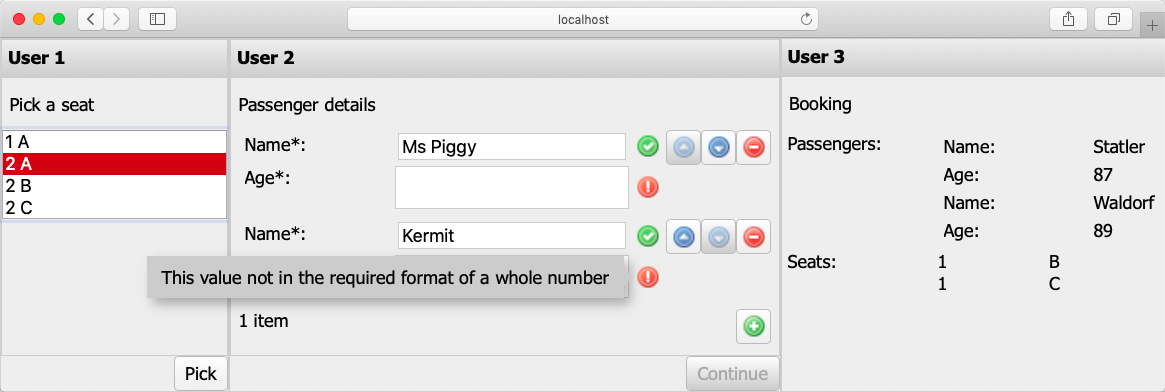
\includegraphics[width=\columnwidth]{figures/flight-booking.png}
  \caption{
    Running web application of the flight booking example using a translation to \ITASKS,
    a \TOP implementation.
    It shows three users booking a flight simultaneously.
    The first user entered name and age and continued to picking seats.
    The second is entering details of two passengers.
    The ages are not filled in, and therefore the \TS{Continue} button is disabled.
    The third user finished a booking.
    Note the first user can't pick seats \smallcaps{1b} and \smallcaps{1c} any more.
    Also, the message bubble shows it is only allowed to enter an integer in the \TS{age} field.
  }
  \label{fig:flight-booking}
\end{figure}

% !TEX root=../icfp2019.tex



\section{Intuition}
\label{sec:intuition}

This section gives an overview over the core concepts of task-oriented programming.

The central objective of \TOP is to \emph{coordinate collaboration}.
The basic building blocks of \TOPHAT for expressing collaboration are task combinators.
They express ways in which people can work together.
Tasks can be executed after each other, at the same time, or conditionally.
This motivates the combinators step, parallel, and choice.

\begin{example}[Breakfast]
\label{exm:breakfast}

The following program shows the different collaboration operators in action.
Users have a choice ($\Xor$) whether they want tea or coffee.
They always get an egg.
The drink and the food are prepared in parallel ($\And$).
When drink and food are prepared, users can step ($\Next$) to eating the results.

\lstset{emph={makeDrink,makeFood}}

% \begin{TASK}
%   let makeBreakfast : Task Drink -> Task Food -> Task Unit =
%     \makeDrink. \makeFood. makeDrink <&> makeFood >>? \<<d, f>>. eat d f
%   let main : Task Unit =
%     makeBreakfast (makeTea <?> makeCoffee) makeEgg
% \end{TASK}

\begin{TASK}
  let makeBreakfast : Task Drink -> Task Food -> Task <<Drink,Food>> =
    \makeDrink. \makeFood. makeDrink <&> makeFood in
  makeBreakfast (makeTea <?> makeCoffee) makeEgg >>? enjoyBreakfast
\end{TASK}

% \begin{TASK}
%   let makeBreakfast : Task Drink -> Task Food -> Task Breakfast =
%     \makeDrink. \makeFood. makeDrink <&> makeFood
%   let main : Task Unit =
%     makeBreakfast (makeTea <?> makeCoffee) makeEgg >>? \breakfast. eat breakfast
% \end{TASK}

The way the combinators are defined matches real life closely.
When we want to have breakfast, we have to complete several other tasks first before we can do so.
We decide what we want to have and then prepare it.
We can prepare the different items we have for breakfast in parallel, but not at the same time.
For example, it is impossible to scramble eggs, and put on the kettle for tea simultaneously.
Instead, what is meant by parallel is that the order in which we do tasks and the smaller tasks that they are composed of, does not matter.
\fixme{Alejandro has placed a line and exclamation under this sentence. I'm not sure what to do here.}
Then finally, only when every item we want to have for breakfast is ready, can we sit down and enjoy it.
\end{example}



\subsection{Tasks are reusable}

Tasks are modular in the following ways.
First, larger tasks are composed from smaller ones.
Second, tasks are first-class, they can be arguments and results of functions.
Third, tasks can be values of other tasks.
These aspects make it possible for programmers to model custom collaboration patterns.

\Cref{exm:breakfast} demonstrates how tasks can be parameterised by other tasks: \TS{makeBreakfast} is a collaboration pattern that always works the same way, regardless of which food and drink are being prepared.



\subsection{Tasks are driven by user input}

Input events drive evaluation of tasks.
When the system receives a valid event, it applies the event to the current task, which results in a new task.
In this way the system communicates with the environment.
Input events are synchronous.
We assume systems react instantaneous to each such event.

In \TOPHAT, editors are the basic method of communication with the environment.
There are different editors, denoted by different box symbols.
An editor of the form $\Edit v$, where $v$ is of type $\tau$, reacts to two kinds of events:
Change events $v$ with a value of type $\tau$ and clear events $\Empty$ which empty the editor.
This results in a typed empty editor $\Enter \tau$, which is annotated with the same type.
\fixme{Alejandro: unclear} %Nico: He has marked the above paragraph as being unclear.


The sole purpose of editors is to interact with users by remembering the last value that has been sent to them.
There are no output events.
As values of editors can be observed, for example by a user interface, editors serve as facilities for both input and output.
An empty editor $\Enter \tau$ stands for a prompt to input data, while a filled editor can be seen either as outputting a value, or as an input that comes with a default value.

\begin{example}[Vending machine]
\label{Vending machine}

This example demonstrates external communication and choice.
It is a vending machine that dispenses a biscuit for one coin and a chocolate bar for two coins.
\begin{TASK}
  let vend : Task Snack = enter Int >>? \n. if n == 1 then edit Biscuit
    else if n == 2 then edit ChocolateBar
    else fail
\end{TASK}
The editor $\Enter \Int$ asks the user to enter an amount of money.
This editor stands for a coin slot in a real machine that freely accepts and returns coins.
There is a continue button that is initially disabled, due to the fact that the left hand side of the step combinator has no value.
When the user has inserted exactly 1 or 2 coins, the continue button becomes enabled.
When the user presses the continue button, the machine dispenses either a biscuit or a chocolate bar, depending on the amount of money.
Snacks are modelled using a custom data type.

\end{example}

\fixme{Alejandro: What is a value? What is a type?}

\subsection{Tasks can be observed}

Several observations can be made about tasks.
One of those is determining the value of a task $\Value(t)$.
% \fixme{Should we change the type of Value to Maybe v? Both johan and alejandro mention that it is not completely clear to them.}
% I don't think that we should use Maybe. We should use the term partial function and bottom. -- mkl
Not all tasks have a value, for example the empty editor $\Enter \tau$, which makes $\Value$ a partial function.
For example, $\Value(\Edit 5) = 5$, $\Value(\Enter \Int) = \bot$.

Another observation is the set of events a task can react to.
This is important for generating user interfaces.
For example, the task $\Edit 5$ can react to value events $v$ and empty events $\Empty$.

In order to render a user interface, the system needs to observe a task's user interface.
This is done compositionally.
User interfaces of combined tasks are composed of the user interfaces of the components.
For example of two tasks combined with a step combinator, only the left hand side is rendered.
Two parallel tasks are rendered next to each other.

In order for the system to actually render a task, it needs to observe the task's value, possible inputs, and user interface.
With this information, the system can then display the current state of the task, together with buttons that show the actions a user can engage in.

The final observation is to determine whether a task results in $\Fail$ (failure).
The step combinator $\Next$ and the choice combinator $\Xor$ use this to prevent users from picking a failing task.




\subsection{Tasks are never done}

Tasks never terminate, they always keep reacting to events.
Editors can always be changed or cleared, and step combinators move on to new tasks.

In a step $t \Next e$, the decision to move on is taken by $\Next$, not by $t$.
The decision is based on a speculative evaluation of $e$.
The step combinators in $t \Then e$ and $t \Next e$ pass the value $v$ of $t$ to the continuation $e$.
Both steps act like $t$ as long as the step is guarded.
A step is guarded if either the left task has no value, or the speculative evaluation $e\ v$ yields $\Fail$.
Once it becomes unguarded, the step continues as $e\ v$.
The task $t \Next e$ additionally requires a continue event $\Continue$ to proceed.
Speculative evaluation is designed so that possible side effects are undone.

The step combinators give rise to a form of internal communication:
They represent data flow that \emph{follows} control flow.



\subsection{Tasks can share information}

The step combinator is one form of internal communication, where task values are passed to continuations.
Another form of internal communication is shared data.
Shared data enables data flow \emph{across} control flow, in particular between parallel tasks.
Shared data sources are assignable references whose changes are immediately visible to all tasks interested in them.
Users can not directly interact with shared data, a shared editor is required for that.
If $r$ is a reference of type $\tau$, then $\Update r$ is an editor whose value is that of $r$.

The semantics of \TOPHAT requires all updates to shared data and all enabled internal steps to be processed before any further communication with the environment can take place.


\begin{example}[Cigarette smokers]

The cigarette smokers problem \cite{books/Downey08LBOS} is a surprisingly tricky synchronisation problem.
We study it here because it demonstrates the capabilities of guarded steps.
% The problem requires waiting for two conditions, waking up only if both conditions are satisfied.
The problem is stated as follows.
In order to smoke a cigarette, three ingredients are required: tobacco, paper, and a match.
There are three smokers, each having one of the ingredients and requiring the other two.
There is an agent that randomly provides two of the ingredients.
The difficulty lies in the requirement that only the smoker may proceed whose missing ingredients are present.

Downey models availability of the ingredients with a semaphore for each ingredient.
The agent randomly signals two of the three semaphores.
The solution proposed by Downey involves an additional mutex, three additional semaphores, three additional threads called \emph{pushers}, and three regular Boolean variables.
The job of the pushers is to record availability of their ingredient in their Boolean variable, and check availability of other resources, waking the correct smoker when appropriate.

The details of the solution are not important here.
What is important is that the implementation of what is essentially deadlock-free waiting for two semaphores requires a substantial amount of additional synchronisation, together with non-trivial conditional statements.

\TOPHAT allows a simple solution to this problem, using guarded steps.
Steps can be guarded with arbitrary expressions, and the parallel combinator can be used to watch two shared editors at the same time.
Let \TS{match}, \TS{paper}, and \TS{tobacco} be references to Booleans.
The smokers are defined as follows.
\begin{TASK}
  let continue = \<<x,y>>. if x /\ y then smoke else fail in
  let tobaccoSmoker = (update match <&> update paper) >>? continue in
  let paperSmoker = (update tobacco <&> update match) >>? continue in
  let matchSmoker = (update tobacco <&> update paper) >>? continue
\end{TASK}
When the agent supplies two of the ingredients by setting the respective shares to \TS{True}, only the step of the smoker that waits for those becomes enabled.

\end{example}



\subsection{Tasks are predictable}

Let $t_1$ and $t_2$ be tasks.
The parallel combination $t_1 \And t_2$ stands for two independent tasks carried out at the same time.
This operator introduces interleaving concurrency.
For the system it does not matter if the tasks are executed by two people actually in parallel, or by one person who switches between the tasks.
The inputs sent to the component tasks are interleaved into a serial stream, which is sent to the parallel combinator.
We assume that such a serialization is always possible.
The tasks are truly independent of each other, all interleavings are permitted.
The environment must prefix events to $t_1$ and $t_2$ by $\First$ (first) and $\Second$ (second) respectively.
This unambiguously renames the inputs, removing any source of nondeterminism.

With concurrency comes the need for synchronisation, in situations where only some but not all interleavings are desired.
The basic method for synchronisation in \TOPHAT is built into the step combinator.
The task $t \Next e$ can only continue execution when two conditions are met:
Task $t$ must have a value $v$, and $e\ v$ must not evaluate to $\Fail$.
Programmers can encode arbitrary conditions in $e\ v$, which are evaluated atomically between interaction steps.
This allows a variety of synchronisation problems to be solved in an intuitive and straight-forward manner.

\Citet{books/Hoare85CSP} states that nondeterminism is only ever useful for \emph{specifying} systems, never for implementing them.
\TOPHAT is meant solely for implementation and does not have any form of nondeterminism.
Input events for parallel tasks are disambiguated, internal steps have a well-defined evaluation order, and internal choice is left-biased.

% \lstset{emph={text}}
% \begin{example}[Abstract submission]
% \label{exm:abstract}
%
% The task of writing an abstract for a conference is never done.
% Let \TS{abstract} be a reference to a string.
%
% % \begin{TASK}
% %   let submit : String -> Task Unit =
% %     \text. delay 30 (sendTo "icfp19@sigplan.org" text)
% %   let write : Task Unit =
% %     edit "Abstract: ..." >>= \abstract. if 500 <= words abstract <= 700 then submit abstract else fail
% % \end{TASK}
%
% \begin{TASK}
%   let submit : Ref String -> Task String = \text. sendTo "icfp19@sigplan.org" text in
%   update abstract <|> delay 30 (submit abstract)
% \end{TASK}
%
% The \TS{delay} task is specified in Example~\ref{exm:delay} in Section~\ref{sec:language}.
%
% \end{example}


\subsection{Recap}

Collaboration in the real world consists of three aspects: communication, concurrency, and synchronisation.
These aspects are reflected in \TOP on a high level of abstraction, hiding the details of communication.
For example, the cigarette smokers communicate with each other, but the programs do not explicitly mention sending or receiving events.

By focussing on collaboration instead of communication, \TOP leads to specifications closer to real-world workflows which, at the same time, can be used to generate distributed, multi-user applications to support such workflows.

% !TEX root=../main.tex



\section{Language}
\label{sec:language}

In this section, we present the constructs of \TOPHAT, our modular interactive workflow language.
We define the host and task language, the types, and the static semantics.
Then we describe the workings of each construct using examples.
These constructs are formalised in \cref{sec:semantics}.

\subsection{Expressions}

\label{sub:expressions}
The host language is a simply typed $\lambda$-calculus, extended with some basic types and \ML-style references.
We use references to represent shared data sources.
The grammar in \cref{fig:language-grammar} defines the syntax of the host language.
It has abstractions, applications, variables, and constants for booleans, integers and strings.
The symbol $\star$ stands for binary operators.
For the result of parallel tasks we need pairs.
Conditionals come in handy for defining guards.
%
References will be used to implement shared editors.
Our treatment of references closely follows the one by \citet{books/Pierce02TAPL}.
Creating a reference using the keyword $\Ref$ yields a location $l$.
While $x$ denotes program variables, $l$ denotes store locations.
Locations are not intended to be directly manipulated by the programmer.
The symbols ! and $:=$ stand for dereferencing and assignment.
The unit value will be used as the result of assignments.

\begin{figure}[h]
  \small
  \usemacro{G-Language-Minimal}
  \caption{Language grammar} \label{fig:language-grammar}
\end{figure}

\label{sub:notation}
We use double quotation marks to denote strings.
Integers are denoted by their decimal representation, and booleans are written $\True$ and $\False$.
We freely make use of the logic operators $\Not$, $\land$, and $\lor$, arithmetic operators $+$, $-$, $\times$, and the string append operator $\pp$.
Furthermore, we use standard comparison operations $<$, $\le$, $\equiv$, $\not\equiv$, $\ge$, and $>$.
The symbol $\star$ stands for any of those.
%
\label{sub:abbreviations}
The notation $e_1; e_2$ is an abbreviation for $(\lambda x:\Unit.\ e_2)\ e_1$, where $x$ is a fresh variable.
The notation $\Let x:\tau = e_1 \In e_2$ is an abbreviation for $(\lambda x:\tau.\ e_2)\ e_1$.

\label{sub:pretasks}
The grammar in \cref{fig:task-grammar} specifies the syntactic category of \emph{pretasks}.
Pretasks are tasks that have unevaluated subexpressions with respect to the host language.
How expressions are evaluated will be discussed in \cref{sec:evaluation}.
Each pretask will be discussed in more detail in the following subsections.
We use open symbols ($\Edit, \Enter, \Next, \Xor$) for tasks that require user input, and closed symbols ($\Update, \Then, \Or$) for tasks that can be evaluated without user input.

\begin{figure}[h]
  \small
  \usemacro{G-Pretasks-Minimal}
  \caption{Task grammar} \label{fig:task-grammar}
\end{figure}



\paragraph{Typing}
\label{sub:typing}

% Typing of our expressions $e$ is as to be expected.
% and won't be given in this document.
\Cref{fig:type-grammar} shows the grammar of types used by \TOPHAT.
It has functions, pairs, basic types, unit, references, and tasks.

\begin{figure}[h]
  \small
  \usemacro{G-Types-Minimal}
  \caption{Type grammar} \label{fig:type-grammar}
\end{figure}

Typing rules are of the form $\RelationT$, which should be read as \enquote{in environment $\Gamma$ and store typing $\Sigma$, expression $e$ has type $\tau$}.
Typing rules for expressions in the host language are presented in the appendix.
The typing rules for pretasks are given in \cref{fig:typing-rules}.
Most typing rules lift the type of their subexpressions into the $\Task$-type.
The typing rules for steps make sure the continuations $e_2$ are functions which accept a well-typed value from the left hand side (\refrule{T-Then}, \refrule{T-Next}).
References, and therefore shared editors, can only be of a basic type so they do not introduce implicit recursion (\refrule{T-Update}).

\begin{figure}[h]
  \small
  \begin{gather*}
    \boxed{\RelationT} \Break
    \userule{T-Edit} \Quad
    \userule{T-Enter} \Quad
    \userule{T-Update} \Break
    \userule{T-Then} \Quad
    \userule{T-Next} \Break
    \userule{T-Fail} \Quad
    \userule{T-And} \Break
    \userule{T-Or} \Quad
    \userule{T-Xor}
  \end{gather*}
  \caption{Typing rules} \label{fig:typing-rules}
\end{figure}



\subsection{Editors}

Programs in \TOPHAT model interactive workflows.
Interaction means communication with end users.
End users should be able to enter information into the system, change it, clear it, reenter it, and so on.
To do this, we introduce the concept of \emph{editors}.
%
Editors are typed containers that either hold a value or are empty.
Editors that have a value can be \emph{changed} or \emph{emptied}.
Empty editors can be \emph{filled}.

% \begin{figure}[h]
%   \centering
%   \includegraphics[width=\columnwidth,page=3]{figures/drawings-crop.pdf}
%   \caption{
%     Possible states of an editor and its transitions.
%     Shared editors cannot be cleared.
%   }
%   \label{fig:editor-state}
% \end{figure}

Editors stand for various forms of input and output, for example widgets in a \GUI, form fields on a webpage, sensors, or network connections.
%
Consider the editor for a person's age from \cref{exm:flight-booking}.
Users can change the value until they are satisfied with it.
Editors are meant to capture this constantly changing nature of user input.
%
The user interface of an editor depends on its type.
This could be an input field for strings, a toggle switch for booleans, or even a map with a pin for locations.
It could also be a parser that tries to parse a line of text to match the type of the editor.


\paragraph{Valued and unvalued editors $(\Edit e, \Enter \tau)$}

Editors that hold an expression $e : \tau$ have type $\Task \tau$.
Empty editors are annotated with a type in order to ensure type safety.
Without type annotations, it would be possible to change the type of an editor, by clearing it and filling it with a value of different type.

\paragraph{Shared editors $(\Update e)$}

Shared editors watch references, lifting their value into the task domain.
If $e$ is a reference $\Reference \tau$, then $\Update e$ is of type $\Task \tau$.
Shared editors cannot be cleared, only changed.

Changes to a shared editor are immediately visible to all shared editors watching the same reference.
Imagine two users, Marco and Christopher, both watching shared editors of the same coordinates.
The editors are visualised as a pin on a map.
When Marco moves his pin, he updates the value of the shared editor, thereby changing the value of the reference.
This change is immediately reflected on Christopher's screen: The pin changes its position on his map.
This way Marco and Christopher can work together to edit the same information.

\label{sub:time}
Two other important use cases for shared editors are sensors and time.
Sensors can be represented as external entities that periodically update a shared editor with their current sensor value.
Similarly, the current time can be stored in a shared editor (\TS{update time}) which is periodically updated by a clock.
The actual sensor and the clock are not modelled in \TOPHAT.
We assume that they exist as external users that send update events to the system.
This allows programmers to write tasks that react to sensor values or timeouts.


\subsection{Steps}

Editors represent atomic units of work.
In this section we look at ways to compose smaller tasks into bigger ones.
Composing tasks can be done in two ways, sequential and parallel.
Parallel composition comes in two variants: combining two tasks (\emph{and}-parallel) and choosing between two tasks (\emph{or}-parallel).
We study sequential composition first, and after that combining and choosing.


\paragraph{Internal and external step $(t \Then e, t \Next e)$}
\label{sub:steps}

Sequential composition has a task $t$ on the left and a continuation $e$ on the right.
External steps ($\Next$) must be triggered by the user, while internal steps ($\Then$) are taken automatically.
The accompanying typing rules are \refrule{T-Then} and \refrule{T-Next}.
According to these rules, the left hand side must be a task $t : \Task \tau_1$, and the right hand side $e : \tau_1 \to \Task \tau_2$ must be a function that, given the task value of $t$, calculates the task with which to continue.

Steps are guarded, which means that the step combinators can only proceed when the following conditions are met.
The left hand side must have a value, only then can the right hand side calculate the successor task.
The successor task must not be $\Fail$, introduced below.
This is enforced on the semantic level, as described in the next section.
The internal step can proceed immediately when these conditions are met.
The external step must additionally receive a continue event $\Continue$.


\begin{example}[Conditional stepping]
\label{exm:conditions}

Consider the following:
\begin{TASK}
  enter Int >>= \n. if n == 42 then edit "Good" else edit "Bad"
\end{TASK}
Initially, the step is guarded because the editor does not have a value.
When users enter an integer, the program continues immediately with either \TS{edit "Good"} or \TS{edit "Bad"}, depending on the input.

\end{example}




\paragraph{Fail $(\Fail)$}
\label{sub:fail}

Fail is a task that never has a value and never accepts input.
The typing rule \refrule{T-Fail} states that it has type $\Task \tau$ for any type $\tau$.
Programmers can use $\Fail$ to tell steps that no sensible successor task can be determined.

\begin{example}[Guarded stepping]

Consider this slight variation on \cref{exm:conditions}:
\begin{TASK}
  enter Int >>= \n. if n == 42 then edit "Good" else fail
\end{TASK}
The user is asked to enter an integer.
As long as the right hand side of $\Then$ evaluates to $\Fail$, the step cannot proceed, and the user can keep editing the integer.
As soon as the value of the left hand side is $42$, the right hand side evaluates to something other than $\Fail$, and the step proceeds to \TS{edit "Good"}.

\end{example}



\begin{example}[Waiting]\label{exm:wait}

\lstset{emph={amount,start,now}}
With the language constructs seen so far it is possible to create a task that waits for a specified amount of time.
To do this,
we make use of a shared editor holding the current time (see \cref{sub:time}),
and a guarded internal step.
\begin{TASK}
  let wait : Int -> Task Unit = \amount : Int.
    update time >>= \start : Int.
    update time >>= \now : Int.
      if now > start + amount then edit <<>> else fail
\end{TASK}
The first step is immediately taken, resulting in \TS{start} to be the time at the moment \TS{wait} is executed.
The second step is guarded until the current time is greater to the start time plus the requested \TS{amount}.

\end{example}



\subsection{Parallel}

A common pattern in workflow design is splitting up work into multiple tasks that can be executed simultaneously.
In \TOPHAT, all parallel branches can progress independently, driven by input events.
This requires inputs to be tagged in order to reach the intended~task. %%XXX: Hack to force `task` on the same line.

There are two ways to proceed after a parallel composition.
One way is to wait for all tasks to produce results and combine those,
the other to pick the first available result.
Both ways introduce explicit forks and implicit joins in \TOPHAT.


\paragraph{Combination $(e_1 \And e_2)$}

A combination of two tasks is a parallel \emph{and}.
It has a value only if both branches have a value.
This is reflected in the typing rule \refrule{T-And},
It shows that if the first task has type $\tau_1$,
and the second has type $\tau_2$,
their combination has the pair type $\tau_1 \times \tau_2$.



\begin{example}[Combining]

The task
\begin{TASK}
  enter Int <&> edit " Batman" >>= \<<n, s>>. edit (replicate n "Na" ++ s)
\end{TASK}
can only step when both editors have values.
When it steps, the continuation uses the pair to calculate the result.

\end{example}


\paragraph{Internal and external choice $(e_1 \Or e_2, e_1 \Xor e_2)$}

Internal choice ($\Or$) is a parallel \emph{or}.
It picks the leftmost branch that has a value.
Its typing rule \refrule{T-Or} states that both branches must have the same type $\Task \tau$.
For example $\Enter \Int \Or \Edit 37$ normalizes to $\Edit 37$, because $\Enter \Int$ doesn't have a value.
Users can work on both branches of an internal choice simultaneously.

External choice ($\Xor$) is different in this regard.
An external choice requires users to pick a branch before continuing with it.
This means users cannot work on the branches of an external choice before picking one.
%XXX: Alejandro: Is this actually implied?
% Ik snap niet zo goed wat Alejandro hier mee bedoelt... --TS


\begin{example}[Delay]
\label{exm:delay}

\lstset{emph={proceed}}

We illustrate the use of internal and external choice by means of
an example that asks users to proceed with a given task or to cancel.
If the user does not make a choice within a given time frame, the program proceeds automatically.
The example makes use of the task \TS{wait} from \cref{exm:wait}.
\begin{TASK}
  let cancel : Task Unit = edit <<>> in
  let delay : Int -> Task Unit -> Task Unit = \n. \proceed.
    (proceed <?> cancel) <|> (wait n >>= \u : Unit. proceed)
\end{TASK}
Note that \TS{delay} is higher-order.
It is a task which takes another task as parameter.

\end{example}

% \subsection{Appointment}
%
%
% It is essential for a workflow system to support multiple collaborators working
% together. Adding this funcitonaltiy to the \TOPHAT language is very
% straightforward. We identify users by means of a name $u$ which we can then use
% to label appointed tasks. The sole purpose of this labelling is to be able to
% tell which inputs are expected from what users. Other than that, it has no
% influence on the semantics. For space reasons, we have have excluded multi-user
% support from this paper.
%
% Mss moeten we het schrijven vanuit het oogpunt van labeling: je kunt labels
% toevoegen aan knoppen, als uitleg bij taken en om gebruikers toe te kennen aan
% taken. Vervolgens zou je iets met die gebruikers kunnen doen: alleen taken voor
% hun weergeven in de UI, alleen inputs voor hun genereren met I etc. Past dat?

\subsection{Annotations}

Tasks can be annotated with additional information.
The system can use this information in various ways.
Possible use cases are labels for the user interface, resource consumption information for static resource analysis, or messages for automatic end-user feedback.
Annotations are not covered in this paper.
Our Haskell implementation of \TOPHAT supports annotating tasks with user \ID{}s, so that individual tasks in a large workflow can be assigned to different users.
These annotations are used to filter the user interfaces for each user so that they can only see their part of the workflow.


% For now, we only concentrate on appointing tasks to users,
% which is common in workflow modelling.
%
%
%
% \paragraph{Appoint $(u \At e)$}
%
% Users are identified by a name $u$ which is a string.
% They can be appointed tasks by means of the $\At$ combinator.
% The sole purpose of this labelling is to be able to tell users which inputs are expected of them.
% In \cref{sec:handling}, a function is described to calculate which users can take what actions.
% Other than this function, the appointment of tasks has no influence on the semantics.
% All semantic rules in \cref{sec:semantics} simply continue with their operations as if the label was not there.

% !TEX root=../icfp2019.tex



\section{Semantics}
\label{sec:semantics}

In this section we formalise the semantics of the language constructs described in \cref{sec:language}.
We organise this by following the structure of the language.

Firstly, the task language is embedded in a simply typed lambda calculus.
This requires a specification of the evaluation of terms in the host language, and how it handles the task language.

Secondly, there are two ways to drive evaluation of task expressions, internally by the system itself, and externally by the user.
This is done in two additional semantics, one for the internal normalisation of tasks, and another for the interaction with the end user.

One of our explicit goals is to keep the semantics for evaluation and normalisation separate,
to not mix general purpose programming notions with workflow specific semantics.
This is achieved by letting tasks be values in the host language.

The three main layers of semantics are thus \emph{evaluation}, \emph{normalisation}, and \emph{interaction}.
The semantics, together with \emph{observations}, will be discussed in the following subsections.
\Cref{fig:semantic-functions} shows the relation between the semantics.
It also shows that there are two helper semantics, \emph{handle} and \emph{stride}.

\begin{figure}[h]
  \centering
  \includegraphics[width=0.6\columnwidth,page=5]{figures/drawings-crop.pdf}
  \caption{
    Semantic functions defined in this report and their relation.
  }
  \label{fig:semantic-functions}
\end{figure}

We use the convention that downward arrows are big-step semantics, and rightward arrows are small-step semantics.



\subsection{Evaluating expressions}
\label{sec:evaluation}

The host language evaluates expressions using a big-step semantics.
Evaluating an expression $e$ in state $s$ into a value $v$ in state $s'$ is denoted by $\RelationE$.
To ease reasoning about references, we choose a call-by-value evaluation strategy.

\Cref{fig:value-grammar} shows values with respect to the evaluation semantics.
Tasks are values, and the operands of task constructors are evaluated eagerly.
Exceptions to this are steps and external choice, where some or all of the operands are not evaluated.

\begin{figure}[h]
  \small
  \usemacro{G-Values-Compact}
  \caption{Value grammar} \label{fig:value-grammar}
\end{figure}

The rules to evaluate expressions $e$ do not differ from standard work, except for the task constructs.
The evaluation rules for tasks can be deduced from the value grammar.
They are given in the appendix.

% \begin{figure}[h]
%
%   \begin{gather*}
%     \userule{E-Edit} \Quad
%     \userule{E-Enter} \Quad
%     \userule{E-Update} \Break
%     \userule{E-Then} \Quad
%     \userule{E-Next} \Break
%     \userule{E-And} \Quad
%     \userule{E-Or} \Break
%     \userule{E-Xor} \Quad
%     \userule{E-Appoint} \Quad
%     \userule{E-Fail}
%   \end{gather*}
%
%   \caption{Evaluation semantics for pretasks} \label{}
% \end{figure}


\subsection{Task observations}

% \begin{figure*}[b]
%   \small
%   \usemacro{O-Value-Compact} \hfill \usemacro{O-Failing-Compact} \hfill \usemacro{O-Inputs-Compact}
%   \caption{Values} \label{fig:observation-value}
% \end{figure*}

The normalisation and interaction semantics make use of observations on tasks.
Observations are semantic functions on the syntax tree of tasks.
There are four semantic functions: $\Value$ for the current task value, $\Failing$ to determine if a task fails, $\Inputs$ for the currently accepted input events, and a function for generating user interfaces.
The semantics make use of $\Value$ and $\Failing$, while $\Inputs$ is used for proving safety.
The function for user interfaces is not used by the semantics, but by our implementation.
It is only described in passing here.




\paragraph{Observable values $(\Value)$}

Task values are used by steps to calculate the successor task.
Filled editors are tasks which contain values, as are shared editors.
Unvalued editors do not contain values, neither does the fail task.
These facts propagate through all other task constructors.
The partial function $\Value$ associates a value $v$ to tasks $t$ where possible.
Its definition is given in \cref{fig:observation-value}.

\begin{figure}[h]
  \small
  \usemacro{O-Value}
  \caption{Values} \label{fig:observation-value}
\end{figure}

Internal and external steps do not have an observable value, because calculating the value would require evaluation of the continuation.
Parallel composition only has a value when both branches have values, in which case these values are paired.
Internal choice has a value when one of the branches has a value.
When both branches have a value, it takes the value of the left branch.
External choice does not have a value because it waits for user input.



\paragraph{Failing $(\Failing)$}

In \cref{sub:fail} we introduced $\Fail$ to stand for an impossible task.
Combinations of tasks can also be impossible.
Take for example the parallel composition of two fails ($\Fail \And \Fail$).
This expression is equivalent to $\Fail$, because it can not handle input and can not be further normalised.

This intuition is formalised by the function $\Failing$ in \cref{fig:observation-failing}.
It determines whether a task is impossible.
Such tasks are called \emph{failing}.

\begin{figure}[h]
  \small
  \usemacro{O-Failing}
  \caption{Failing} \label{fig:observation-failing}
\end{figure}

Steps whose left hand sides are failing can never proceed because of the lack of an observable value.
Therefore they are itself failing.
The internal choice of two failing tasks is failing.
External choices let the user pick a side and only then evaluate the corresponding subexpression.
To determine if an external choice is failing, it needs to peek into the future to check if both subexpressions are failing.
Annotations are failing only if the inner task is failing.



\paragraph{User interface}

%\fixme{Add $\UserInterface$ to appendix and refer.}
\TOPHAT is designed such that a user interface can be generated from a task's syntax tree.
A possible graphical user interface is shown in \cref{fig:flight-booking}, where tasks are rendered as \HTML pages.
Editors are rendered as input fields,
external choices are represented by two buttons,
and parallel tasks are rendered side by side.
Steps only show the interface of their left hand side.
In case of an external step they are accompanied by a button.
When the guard condition of a step is not fulfilled, the button is disabled.



\subsection{Normalising tasks}
\label{sec:normalise}

The normalisation semantics is responsible for reducing expressions of type $\Task$ until they are ready to handle input.
It is a big-step semantics, and makes use of evaluation of the host language.
We write $\RelationN$ to describe that
an expression $e$ in state $s$ normalises to task $t$ in state $s'$.

Normalisation rules are given in \cref{fig:normalisation-semantics}.
Both rules ensure that expressions are first evaluated by the host language ($\evaluate$), and then by the stride semantics ($\stride$).
These two actions are repeated until the resulting state and task stabilise.

\begin{figure}[h]
  \small

  \boxed{\RelationN}
  \begin{gather*}
    \userule{N-Done} \Break
    \userule{N-Repeat}
  \end{gather*}
  \caption{Normalisation semantics} \label{fig:normalisation-semantics}

\end{figure}

The split between striding and normalisation is due to mutable references.
Consider the following example, where $s=\set{l\mapsto\False}$.
\begin{TASK}
  (update l >>= \x:Bool. if x then e else fail) <&> (l := True; edit <<>>)
\end{TASK}
\refrule{S-And} reduces this expression in one step to
\begin{TASK}
  (update l >>= \x:Bool. if x then e else fail) <&> (edit <<>>)
\end{TASK}
with $s'=\set{l\mapsto\True}$.
This expression is not normalised, because the left task can take a step.
The issue here lies in the fact that the right task updates $l$.
To overcome this problem, the \refrule{N-Done} and \refrule{N-Repeat} rules ensure that striding is applied until the state $s$ becomes stable and no further normalisation can take place.

The striding semantics is responsible for reducing internal steps and internal choices.
A stride from task $t$ in state $s$ to $t'$ in state $s'$ is denoted by $\RelationS$.
The rules for striding are given in \cref{fig:striding-semantics}.
Tasks like editors, fail and external choice are not further reduced.
For external choice and parallel there are congruence rules.

\begin{figure}[h]
  \small

  \begin{gather*}
    \boxed{\RelationS}
  \end{gather*}

  \paragraph{Step}
  \begin{align*}
    \userule{S-ThenStay} \Quad
    & \userule{S-ThenFail} \Break
    & \userule{S-ThenCont}
  \end{align*}

  \paragraph{Choose}
  \begin{align*}
    \userule{S-OrLeft} \Quad
    & \userule{S-OrRight} \Break
    & \userule{S-OrNone}
  \end{align*}

  \paragraph{Ready}
  \begin{gather*}
    \userule{S-Edit} \Quad \userule{S-Fill} \Quad \userule{S-Update} \Quad
    \userule{S-Fail} \Quad \userule{S-Xor}
  \end{gather*}

  \paragraph{Congruence}
  \begin{gather*}
    \userule{S-Next} \Quad
    \userule{S-And}
    %\userule{S-Appoint}
    % \userule{S-Eval}
  \end{gather*}

  \caption{Striding semantics} \label{fig:striding-semantics}
\end{figure}



\paragraph{Principles of stepping}
\label{sub:stepping-principles}

Stepping away from task $t_1$ can only be performed when
$t_1$ has a value: $\Value(t_1) = v_1$.
Only then can a new task $t_2$ be calculated from the expression $e$.
On top of that, $t_2$ must not be failing: $\neg\Failing(t_2)$.

These principles lead to the stepping rules in \cref{fig:striding-semantics}.
\refrule{S-ThenStay} does nothing,
because the left side does not have a value.
\refrule{S-ThenFail} covers the case that
the left side has a value but the calculated successor task is failing.
This rule uses the semantics of the host language to evaluate the application $e_2\ v_1$.
When all required conditions are fulfilled, \refrule{S-ThenCont} allows stepping to the successor task.



\paragraph{Principles of choosing}
\label{sub:choosing-principles}

Choosing between two tasks $t_1$ and $t_2$ can only be done when
at least one of them has a value: $\Value(t_1) = v_1 \lor \Value(t_2) = v_2$.
When both have a value, the left task is chosen.
When none has a value, none can be chosen.
These principles lead to the rules \refrule{S-OrLeft}, \refrule{S-OrRight}, and \refrule{S-OrNone},
which encode that the choice operator picks the leftmost task that has a value.



\subsection{Handling user inputs}
\label{sec:handling}

The handling semantics is the outermost layer of the stack of semantics.
It is responsible for performing external steps and choices, and for changing the values of editors.
The rules of the interaction semantics are given in \cref{fig:interaction-semantics}.
The semantics is only applicable to normalised $t$.
Sending an input event $i$ to a task $t$ first handles the event and then prepares the resulting task for the next input by normalising it.

\begin{figure}[h]
  \small
  \begin{gather*}
    \boxed{\RelationI} \Break
    \userule{I-Handle}
  \end{gather*}
  \caption{Interaction semantics} \label{fig:interaction-semantics}
\end{figure}

Inputs $i$ are formed according to the grammar in \cref{fig:input-grammar}.
%
There is a function $\Inputs$ which calculates the possible input events a given task expects.
It takes a normalised task and a state and returns a set of inputs that can be handled.
The definition of this function is listed in \cref{fig:observation-input}.

\begin{figure}[h]
  \small
  \usemacro{G-Inputs-Compact}
  \caption{Input grammar} \label{fig:input-grammar}
\end{figure}

\begin{figure}[h]
  \small
  \usemacro{O-Inputs}
  \caption{Inputs} \label{fig:observation-input}
\end{figure}

Handling input is done by the \emph{handling} semantics shown in \cref{fig:handling-semantics}.
It is a small step semantics with labelled transitions.
It takes a task $t$ in a state $s$ and an input $i$, and yields a new task $t'$ in a new state $s'$.

\begin{figure}[h]
  \small

  \begin{gather*}
    \boxed{\RelationH}
  \end{gather*}

  \paragraph{Editing}
  \begin{gather*}
    \userule{H-Change} \Quad
    \userule{H-Empty} \Break
    \userule{H-Fill} \Quad
    \userule{H-Update}
  \end{gather*}

  \paragraph{Continuing}
  \begin{gather*}
    \userule{H-Next} \Break
    \userule{H-PickLeft} \Quad
    \userule{H-PickRight}
  \end{gather*}

  \paragraph{Passing}
  \begin{gather*}
    \userule{H-PassThen} \Quad \userule{H-FirstAnd} \Quad \userule{H-FirstOr} \Break
    \userule{H-PassNext} \Quad \userule{H-SecondAnd} \Quad \userule{H-SecondOr}
  %  \userule{H-Appoint}
  \end{gather*}

  \caption{Handling semantics} \label{fig:handling-semantics}
\end{figure}

%FIXME: Revert rule names in front to normal sentences?
\refrule{H-Change},
\refrule{H-Empty},
\refrule{H-Fill},
\refrule{H-Update}:
Input events $v$ and $\Empty$ are used to change the value of editors and empty them.
Editors only accept values of the correct type.

\refrule{H-Next}:
The $\Continue$(ontinue) action triggers an external step.
As with internal stepping, this is only possible if the left side has a value and the continuation is not failing.

\refrule{H-PickLeft},
\refrule{H-PickRight}:
$\Left$ and $\Right$ are used to pick the left or right option of an external choice.

\refrule{H-PassThen},
\refrule{H-PassNext}:
The step combinators pass all events other than $\Continue$ to the left side.

\refrule{H-FirstAnd},
\refrule{H-SecondAnd},
\refrule{H-FirstOr},
\refrule{H-SecondOr}:
Inputs $\First$(irst) and $\Second$(econd) are used to direct inputs to the correct branch of parallel combinations.



\subsection{Implementation}

The semantics have been implemented in the Idris programming language \cite{journals/jfp/Brady13}.
We use techniques presented by \textcite{journals/entcs/JaskelioffGH11}, \textcite{journals/jfp/Swierstra08}, and \textcite{school/maktoberdorf/PeytonJones01}.
% Such an implementation increases the confidence in the correctness and completeness of the semantics.
The source code can be found on GitHub.\footnote{\url{http://github.com/XXX/XXX}}
% A proof of concept implementation in Haskell is also available, showing that \TOPHAT can be implemented without dependent types.
A command-line interface is part of this implementation.
It prompts users to type input events, which get parsed and processed by the interaction semantics.

Also, we mad an implementation of \TOPHAT combinators into \ITASKS,
so that \TOPHAT specifications can be compiled to runnable applications.
This shows that \TOPHAT is a subset of \ITASKS.

% !TEX root=../icfp2019.tex



\section{Properties}
\label{sec:properties}



% \subsection{Safety}

In order to validate our semantics, we show that our evaluation, normalisation
and handling semantics is type preserving. We additionally prove a progress
theorem for our small-step handling semantics.

Additionally, we show that the normalisation semantics is a big-step semantics.
%XXX: Alejandro: ?
% Niks meer mee doen, was voor PLDI reviewers duidelijk genoeg. --TS
While at first sight, this might seem obvious, the fact that we are dealing with
state complicates matters.

We show that our failing function $\Failing$ indeed only indicates expressions
that can not be normalised and that allow no further interaction.

Finally, we prove that the function to compute all possible inputs $\Inputs$ is sound and complete.



\subsection{Type preservation}
\label{sub:preservation}

We show that the following three preservation Theorems hold.

\begin{theorem}[Type preservation under evaluation]
  % For all well typed expressions $e$ and states $\sigma$,
  For all expressions $e$ and states $\sigma$
  such that $\Gamma,\Sigma \infers e:\tau$ and $\Gamma,\Sigma \infers \sigma$,
  if $e,\sigma \evaluate e',\sigma'$,
  then $\Gamma,\Sigma \infers e':\tau$ and $\Sigma \infers \sigma'$.
  \label{thm:pres-eval}
\end{theorem}

Where $\Sigma \infers \sigma$ means that for all $l\in \sigma$, it holds that
$\Sigma(l)=\Gamma,\Sigma\infers \sigma(l)$.

\Cref{thm:pres-eval} is shown to be correct by induction over $e$. The full
proof can be found in the appendix.


Moving on, we show that normalisation also preserves types, by showing that the following Theorem holds.

\begin{theorem}[Type preservation under normalisation]
  % For all well typed expressions $e$ and states $\sigma$,
  For all expressions $e$ and states $\sigma$
  such that $\Gamma,\Sigma \infers e:\Task\tau$ and $\Sigma \infers \sigma$,
  if $e,\sigma \normalise e',\sigma'$,
  then $\Gamma,\Sigma \infers e':\Task\tau$ and $\Sigma \infers \sigma'$.
  \label{thm:pres-norm}
\end{theorem}

Since this semantics makes use of the value function $\Value$ and the striding semantics $\stride$,
we first need to show that preservation also holds for these two semantics.

\begin{lemma}[Task value preserves types]
  % For all well typed expressions $e$ and states $\sigma$,
  For all expressions $e$ and states $\sigma$
  such that $\Gamma,\Sigma \infers e:\Task\tau$ and $\Sigma \infers \sigma$,
  if $\Value{(e,\sigma)}=v$,
  then $v:\tau$.
  \label{lem:presvalue}
\end{lemma}

\begin{lemma}[Striding preserves types]
  For all expressions $e$ and states $\sigma$
  such that $\Gamma,\Sigma \infers e:\Task\tau$ and $\Sigma \infers \sigma$,
  if $e,\sigma \stride e',\sigma'$,
  then $\Gamma,\Sigma \infers e':\Task\tau$ and $\Sigma \infers \sigma'$.
  \label{thm:pres-stride}
\end{lemma}

\Cref{lem:presvalue} and \cref{thm:pres-stride} are proven in the
appendix by induction over $e$. This subsequently allows us to prove
\Cref{thm:pres-norm}, again by induction over $e$.

This brings us finally to the type preservation property of the handling semantics.

\begin{theorem}[Type preservation under handling]
  % For all well typed expressions $e$, states $\sigma$, and inputs $i$,
  For all expressions $e$, states $\sigma$ and inputs $i$
  such that $\Gamma,\Sigma \infers e:\Task\tau$ and $\Sigma \infers \sigma$,
  if $ e,\sigma \handle{i} e',\sigma'$,
  then $\Gamma,\Sigma\infers e':\Task\tau$ and $\Sigma\infers \sigma'$.
  \label{thm:pres-handle}
\end{theorem}

And again, this is proven by induction over $e$.

From \cref{thm:pres-handle} and \cref{thm:pres-norm} we directly
obtain that the driving semantics also preserves types.

\subsection{Progress}

A well-typed term of a task type is guaranteed to progress after normalisation,
unless it is failing.

We define what we mean with progress in \cref{thm:prog-norm}.
\begin{theorem}[Progress under handling]
  For all well typed expressions $e$ and states $\sigma$,
  % For all expressions $e$ and states $\sigma$
  % such that $\Gamma,\Sigma \infers e:\Task\tau$ and $\Sigma \infers \sigma$,
  if $e,\sigma \normalise e',\sigma'$,
  then either $\Failing(e', \sigma')$
  or there exist $e''$, $\sigma''$, and $i$ such that $e',\sigma'\handle{i} e'',\sigma''$.
  \label{thm:prog-norm}
\end{theorem}

Where a well typed expression $e$ means that $\Gamma,\Sigma\infers e:\tau$ for
some type $\tau$, and a well typed state means that $\Sigma\infers \sigma$.

If an expression $e$ and state $\sigma$ are well-typed, then after normalisation, the pair $e',\sigma'$
either fails, or there exists some input $i$ that can be handled by it under the handling semantics.
In order to prove this Theorem, we require an additional theorem.

% \paragraph{Failing}

We need to show that the failing function $\Failing$ behaves as desired.

\begin{theorem}[Failing means no interaction possible]
  For all well typed expressions $e$ and states $\sigma$,
  % For all expressions $e$ and states $\sigma$
  % such that $\Gamma,\Sigma \infers e:\Task\tau$ and $\Sigma \infers \sigma$,
  and $e,\sigma \normalise e',\sigma'$,
  we have that $\Failing(e',\sigma') = \True$,
  if and only if there is no input $i$
  such that $e',\sigma'\handle{i} e'',\sigma''$ for some $e''$ and $\sigma''$.
  \label{thm:failing}
\end{theorem}

The Theorem above states that an expression $e$ and state $\sigma$ are failing, if,
after normalisation, there exists no input that can be handled by it.
We prove the theorem to be true by induction on $e'$.

% \paragraph{Proof}

We now have the ingredients to prove \cref{thm:prog-norm}.

\begin{proof}
  Given $\Gamma,\Sigma\infers e:\Task\tau$ and $\Sigma\infers \sigma$ and after
  normalisation $e,\sigma \normalise e',\sigma'$, we find ourselves in either one of the
  following situations:

  There exists an $i$ such that $e',\sigma'\handle{i} e'',\sigma''$.

  There does not exist an $i$ such that $e',\sigma'\handle{i} e'',\sigma''$. In this case, we
  know that $\Failing(e',\sigma')$ must be true, by \cref{thm:failing}.
\end{proof}



\subsection{Soundness and Completeness of Inputs}

In order to validate the function that calculates all possible inputs $\Inputs$,
we want to show that the set of possible inputs it produces is both sound and complete with respect to the handle semantics.
By sound we mean that all inputs in the set of possible inputs can actually be handled by the handle semantics,
and by complete we mean that the set of possible inputs contains all inputs that can be handled by the handle semantics.
\Cref{thm:safety-i} expresses exactly this property.

\begin{theorem}[Inputs function is sound and complete]
  For all well typed expressions $e$, states $\sigma$, and inputs $i$,
  % For all expressions $e$, states $\sigma$, and inputs $i$
  % such that $\Gamma,\Sigma \infers e:\tau$ and $\Sigma \infers \sigma$,
  we have that $i \in \Inputs{(e,\sigma)}$ if and only if $e,\sigma \handle{i} e',\sigma'$.
  \label{thm:safety-i}
\end{theorem}

We prove the above theorem by induction over $e$. The proof is listed in the
appendix.

% !TEX root=../icfp2019.tex



\subsection{Outlook}

At this point we have specified a formal language for task-oriented programming,
given its semantics, and proved its safety.
The main motive to formalise this paradigm, is to be able to reason about tasks.
In future work, we plan on utilising the formalisation to do so.

Firstly, we would like to express properties of tasks and prove them.
For example, one would like to prove that, no matter what, in Example~\ref{exm:abstract} an abstract is always submitted.
Secondly, we would like explore what it means for two tasks to be equal.
One could have noticed that some operators have a monadic or applicative feeling.
The combination of $\And$ and $\Edit$ could form a (lax) monoidal functor,
$\Or$ is similar to applicative choice,
and $\Then$ looks like a bind operation.
We need a correct understand of equivalency of tasks,
taking the interactive setting into account,
to prove this.
Thirdly, we do not know yet if the more complex combinators of \ITASKS are expressible in the basic combinators of \TOPHAT.
We implemented \TOPHAT on top of \ITASKS, so we know it is a subset,
but we also know \ITASKS can do more.

% The work presented in this paper describes a formal foundation for task oriented programming.
% For the first time, this programming paradigm has been formalised.
% The formalisation allows us to reason about \TOP and programs written in \TOPHAT.
% So far, we have proven type safety and progress, but this is merely the beginning.
% In future work, we plan on utilising the formalisation to do much more.

% First of all, we would like to show that certain properties hold for individual programs.
% We would also like to be able to define what it means for programs to be equal.

A more in depth description of future work can be found in Section~\ref{sec:conclusions}.

% !TEX root=../icfp2019.tex



\section{Related work}
\label{sec:relatedwork}

\fixme{Intro related work}


\subsection{Task-oriented programming implementations}

\paragraph{iTasks}

As mentioned earlier, iTasks is an implementation of \TOP. iTasks has many
features, and its basic combinators are versatile and powerful. Simpler
combinators are implemented by restricting the powerful ones. This is useful for
everyday programming, where having lots of functionality at one's fingertips is
convenient and efficient.

There have been two previous papers that describe semantics of iTasks, by
\citet{conf/ifl/KoopmanPA08} and \citet{conf/ppdp/PlasmeijerLMAK12}.
Both give a different semantics in the form of minimal implementations of a
subset of the interface of iTasks. These semantics however do not make an
explicit distinction between the host language and task language and they do not
provide a formal semantics, which makes formal reasoning difficult.

\paragraph{mTasks}
\fixme{Hier iets gezelligs over mTasks}
% Our work differs in three major ways.
% First, we make an explicit distinction between the host language and the task
% language, to emphasise their boundaries.
% Second, we make use of separate semantic functions for querying the current task
% value, determining the continuation after an input event, and producing a user
% interface.
% In iTasks and its aforementioned semantics, these are integrated into the
% \CL{Task} datatype.
% Third, our system does not have the notion of task stability.
% When desired, stability can be introduced by the programmer, but the system
% itself makes no use of it.
% We argue that this does not impact the expressiveness of our language.

% mTasks is another implementation of TOP, designed for coordination of IoT devices. \alert{cite MSc Lubbers}
% mTasks has been used in a demonstrator for home automation. \alert{cite MSc Andrade}



\subsection{Worfklow modelling}

Much research has been done into workflow modelling. These works focus on
describing the collaboration between subsystems, rather than the communication
between them.
The systems described here follow a \emph{boxes and arrows} model of specifying workflows.
Control flow, represented by arrows, usually can go unrestricted from anywhere to anywhere else in a workflow.
We see \TOP as the functional programming of workflows, as opposed to this \emph{goto}-style.


\paragraph{Workflow patterns}

Workflow patterns are regarded as special kind of the design patterns in
software engineering. They identify recurring patterns in workflow systems, much
like the combinators defined by \TOPHAT. Work by \citet{journals/dpd/AalstHKB03}
defines a comprehensive list of these
pattens, and examines their availability in industry workflow software.
Workflow patterns are usually described in terms of control flow graphs, and no
formal specification is given, which makes comparison and formal reasoning more
difficult.

\paragraph{Workflow Nets}

Workflow Nets~(\WFN)\cite{journals/jcsc/Aalst98} allow for the modelling and analysis
of business processes. They are graphical in nature, and clearly display how
every component is related to each other. A downside of \WFN is that
they do not facilitate higher order constructs and that they are often not
directly executable.

\paragraph{YAWL}

This is not always the case however. A language based on \WFN that is
actually directly executable is \YAWL by \citet{DBLP:journals/is/AalstH05}.
It facilitates modelling and execution of
dynamic workflows, with support for \emph{and}, \emph{or} and \emph{xor} workflow patterns. As
mentioned, \YAWL programs consist of \WFN, and are therefore programmed
visually.

\paragraph{BPEL}

\BPEL~\cite{bpel} is another popular business process language. The standardised
language allows for the specification of actions within business processes,
using an \XML format. Processes specified in \BPEL are executable, just like \YAWL.

\fixme{Is this higher order? What combinators can be used? Other limitations?}


\subsection{Process algebras}

There are two main differences between \TOP and process algebras.
The first is a difference in scope.
Process algebras focus on modelling the input/output behaviour of processes, by explicitly stating which actions are sent and received at certain points in the program.
The goal of process algebras is formal reasoning about the interaction between processes.
Typically, one wishes to prove properties such as deadlock-freedom, liveness, or adherence to a protocol specification.

The focus of \TOP on the other hand is to model collaboration patterns, with the explicit goal of not having to specify how exactly subtasks communicate.
The declarative specification of data dependencies between subtasks enables \TOP to hide such details.

The second difference concerns internal communication.
There are two forms of communication between tasks: Passing values to continuations and sharing data.
This is different from communication in process algebras, which is based on message-passing.


\paragraph{Similarities}
There are some aspects that are similar in \TOPHAT and process algebras.
Internal communication in Hoare's CSP \cite{books/Hoare85CSP} is introduced with the concealment operator.
The semantics of CSP requires that all concealed actions are handled to exhaustion before any action with the environment can take place.
This is somewhat similar to \TOPHAT, where all enabled internal steps must be taken until the system can react to input events again.
Contrast this with Milner's CCS \cite{books/Milner89CAC}, where concealed actions are visible to the outside as $\tau$-actions, and can be interleaved with external communication.

Another similarity between \TOPHAT and process algebras, or any system with concurrency for that matter, is the need for synchronisation.
Broadly speaking, concurrency means that different parts of a program can interact with the environment independently, in an interleaved manner.
Synchronisation means that only some, but not all, of the possible interleavings are desirable.
The semantics of the step combinators in \TOPHAT, together with the fact that internal communication happens atomically, allows for concise TODO: say that synchronisation in TOPHAT is the best.


\subsection{Reactive programming}

\paragraph{Esterel \& HipHop}

\paragraph{Functional reactive programming}

Functional Reactive Programming (\FRP) is a paradigm to describe dynamic changes of values in a declarative way.
This is done by specifying networks of values, called behaviours, that can depend on each other and on external events.
Behaviours can change over time, or triggered by events.
When a behaviour changes, all other behaviours that depend on it are updated automatically.
The underlying implementation that takes care of the updating usually can tie input devices, like mouse and keyboard, to event streams and behaviours to output facilities, like text fields.
This allows for declarative specifications of applications with user interfaces.

The idea of \FRP was pioneered by \citet{conf/icfp/ElliottH97}.
In the meantime there are many variants and implementations, where reactive-banana \cite{reactive-banana}, FrTime \cite{CooperK04}, and Flapjax \cite{conf/oopsla/MeyerovichGBCGBK09} belong to the most well-known.

\FRP and \TOP are different systems that have different goals in mind.
Whereas \FRP expresses automatically updating data dependencies, \TOP expresses collaboration patterns.
\TOP has no notion of time.
Tasks can not change spontaneous over time, while behaviours can.
Only input events can change task values.
The biggest conceptual difference between a workflow in \TOP and a data network in \FRP is that an event to a task only causes updates up until the next step, while an event in \FRP propagates through the whole network.

That being said, there are some concepts that are similar in \TOP and \FRP.
The \emph{stepper} behaviour, for example, is associated with an event and yields the value of the most recent event.
This is similar to editors in \TOP.
Furthermore, both systems can be used to declaratively program user interfaces, albeit in \FRP the programmer has to construct the \GUI elements manually, and connect inputs and outputs to the correct events and behaviours.
In \TOP graphical user interfaces are automatically derived.


\subsection{Session types}

Session types are a type discipline that can be used to check whether communicating programs conform to a certain protocol.
Session types are expressions in some process calculus that describe the input/output behaviour of such programs.
Session types are useful for programming languages where modules communicate with each other via messages, like \CSP, \PICALC, or Go, to name a few.
The only form of messages in \TOP are input events which drive execution, but modules do not communicate using messages.
Therefore, session types are not applicable to \TOP in the sense used in the literature.

Formal reasoning about \TOP programs is one of our future goals for \TOPHAT.
The ideas and techniques of session types could be useful for specifying that a list of inputs of a certain form leads to desired task values.
The details are a topic for future work.


\subsection{Related web services}


\paragraph{IFTTT}

If This Then That (\IFTTT)~\cite{IFTTT} is a web service that allows users to write and
configure simple conditional statements called applets, that can interact with
web services and IoT devices. These applets can be seen as tiny workflows, that
facilitate collaboration between different services and platforms. The
complexity of the flow is very limited however, and is not geared towards humans
collaborating.

\paragraph{Google forms \& Wufoo}

Google Forms~\cite{googleforms} and SurveyMonkey~\cite{wufoo} (and their various other tools like Wufoo, Precise Polling and Zoomerang) are web based survey administration apps that allows
users to compose forms and gather data from them. They are comparable to \TOP and
iTasks in that they provide an easy way for users to construct forms on the web.
However, Google Forms and Wufoo do not allow users to define what the system
then should do with this information, and can therefore not be regarded as a
workflow or business process modelling systems.

\paragraph{Chorus} % (http://www.chorus-home.org/)

Chorus~\cite{chen2017chorus} is a visual programming environment for online
collaboration apps. The goal of Chorus is to allow users to program their own
application, though which a collective task can be coordinated. Users work on a
preset data-type that drives the behaviour of the user defined applications.

% !TEX root=../pldi2019.tex

\section{Conclusion}

\paragraph{Future work}



% %% Acknowledgments
% \begin{acks}                            %% acks environment is optional
%                                         %% contents suppressed with 'anonymous'
%   %% Commands \grantsponsor{<sponsorID>}{<name>}{<url>} and
%   %% \grantnum[<url>]{<sponsorID>}{<number>} should be used to
%   %% acknowledge financial support and will be used by metadata
%   %% extraction tools.
%   \small
%   % !TEX root=../icfp2019.tex

The authors are grateful to Johan Jeuring, Sjaak Smetsers, and Andreas Vinter-Hviid for fruitful discussions,
and Rinus Plasmeijer, Peter Achten and Pieter Koopman for proofreading.

This research is supported by the Dutch Technology Foundation STW, which is part
of the Netherlands Organisation for Scientific Research (NWO), and which is
partly funded by the Ministry of Economic Affairs.

% \end{acks}


%% Bibliography
\bibliography{bibliography}


%% Appendix
\pagebreak \appendix

% !TEX root=../main.tex

\section{Additional rules}

\subsection{Evaluation rules}

% \begin{figure}

  \begin{gather*}
    \boxed{\RelationE} \Break
    \userule{E-App} \Quad
    \userule{E-IfTrue} \Quad
    \userule{E-Ref} \Break
    \userule{E-IfFalse} \Quad
    \userule{E-Deref} \Quad
    \userule{E-Value} \Quad
    \userule{E-Assign} \Break
    \userule{E-Pair} \Quad
    \userule{E-Edit} \Quad
    \userule{E-Enter} \Quad
    \userule{E-Update} \Quad
    \userule{E-Then} \Break
    \userule{E-Next} \Quad
    \userule{E-And} \Quad
    \userule{E-Fail} \Quad
    \userule{E-Or} \Quad
    \userule{E-Xor}
    %\userule{E-Appoint}
  \end{gather*}

%   \caption{Evaluation semantics} \label{fig:evaluation-semantics}
% \end{figure}

\subsection{Typing rules}

% \begin{figure}[h]

  \begin{gather*}
    \boxed{\RelationT} \Break
    \userule{T-Var} \Quad
    \userule{T-Loc} \Quad
    \userule{T-Pair} \Quad
    \userule{T-Abs} \Quad
    \userule{T-App} \Break
    \userule{T-If} \Quad
    \userule{T-Ref} \Quad
    \userule{T-Deref} \Quad
    \userule{T-Assign}
  \end{gather*}

%   \caption{Additional typing rules}
% \end{figure}

\pagebreak
% !TEX root=../icfp2019.tex

\section{Proofs}

\subsection{Theorem~\ref{thm:pres-eval}}

\begin{proof}
  We prove Theorem~\ref{thm:pres-eval} by induction on $e$:\\

  \case
    {$e=\lambda x:\tau.e, e_1 e_2, x, c, l, e_1 \star e_2,\If{e_1}{e_2}{e_3},\tuple{e_1, e_2},\unit,\Ref e,!e,e_1 := e_2$}
    {Preservation has been proven for these cases by Pierce~\cite{books/Pierce02TAPL}.}

  \case
    {$\userule{E-Edit}$}
    {Given that $\Gamma,\Sigma\infers\Edit e:\Task \tau$ and $\Sigma\infers s$,\refrule{T-Edit} gives us that $\Gamma,\Sigma\infers e:\tau$.
    The induction hypothesis gives us that $e,s\evaluate v,s'$ also preserves, and thus $\Gamma,\Sigma\infers v:\tau$ and $\Sigma\infers s'$.
    Therefore $\Gamma,\Sigma\infers\Edit v:\Task\tau$.}

  \case
    {$\userule{E-Enter}$}
    {Evaluation does not alter $e$ and $s$, therefore this case holds trivially.}

  \case
    {$\userule{E-Update}$}
    {Given that $\Gamma,\Sigma\infers \Edit e:\Task \tau$ and $\Sigma\infers s$, \refrule{T-Update} gives us that $\Gamma,\Sigma\infers e:\Ref \tau$.
    The induction hypothesis gives us that $e,s\evaluate l,s'$ also preserves, and thus $\Gamma,\Sigma\infers l:\Ref\tau$ and $\Sigma\infers s'$.
    Therefore $\Gamma,\Sigma\infers\Update l:\Task\tau$.}

  \case
    {$\userule{E-Fail}$}
    {Evaluation does not alter $e$ and $s$, therefore this case holds trivially.}

  \case
    {$\userule{E-Then}$}
    {Given that $\Gamma,\Sigma\infers e_1\Then e_2:\Task \tau$ and $\Sigma\infers s$, \refrule{T-Then} gives us that $\Gamma,\Sigma\infers e_1:\Task\tau_1$ and $\Gamma,\Sigma\infers e_2:\tau_1 \to \Task \tau$.
    By the induction hypothesis, we know that $e_1,s\evaluate t_1,s'$ preserves and thus $\Gamma,\Sigma\infers t_1:\Task\tau_1$ and $\Sigma\infers s'$.
    Therefore $\Gamma,\Sigma\infers t_1\Then e_2:\Task\tau$.}

  \case
    {$\userule{E-Next}$}
    {Given that $\Gamma,\Sigma\infers e_1\Next e_2:\Task \tau$ and $\Sigma\infers s$, \refrule{T-Next} gives us that $\Gamma,\Sigma\infers e_1:\Task\tau_1$ and $\Gamma,\Sigma\infers e_2:\tau_1 \to \Task \tau$.
    By the induction hypothesis, we know that $e_1,s\evaluate t_1,s'$ preserves and thus $\Gamma,\Sigma\infers t_1:\Task\tau_1$ and $\Sigma\infers s'$.
    Therefore $\Gamma,\Sigma\infers t_1\Next e_2:\Task\tau$.}

  \case
    {$\userule{E-And}$}
    {Given that $\Gamma,\Sigma\infers e_1\And e_2:\Task(\tau_1\times\tau_2)$ and $\Sigma\infers s$, \refrule{T-And} gives us that $\Gamma,\Sigma\infers e_1:\Task\tau_1$ and $\Gamma,\Sigma\infers e_2:\Task\tau_2$.
    By the induction hypothesis, we know that both $e_1,s\evaluate t_1,s'$ and $e_2,s'\evaluate t_2,s''$ preserve and thus $\Gamma,\Sigma\infers t_1:\Task\tau_1$, $\Sigma\infers s'$, $\Gamma,\Sigma\infers t_2:\Task\tau_2$ and $\Sigma\infers s''$.
    Therefore $\Gamma,\Sigma\infers t_1\And t_2:\Task(\tau_1\times\tau_2)$.}

  \case
    {$\userule{E-Or}$}
    {Given that $\Gamma,\Sigma\infers e_1\Or e_2:\Task\tau$ and $\Sigma\infers s$, \refrule{T-Or} gives us that $\Gamma,\Sigma\infers e_1:\Task\tau$ and $\Gamma,\Sigma\infers e_2:\Task\tau$.
    By the induction hypothesis, we have that both $e_1,s\evaluate t_1,s'$ and $e_2,s'\evaluate t_2,s''$ preserve and thus $\Gamma,\Sigma\infers t_1:\Task\tau$, $\Sigma\infers s'$, $\Gamma,\Sigma\infers t_2:\Task\tau$ and $\Sigma\infers s''$.
    Therefore $\Gamma,\Sigma\infers t_1\Or t_2:\Task\tau$.}

  \case
    {$\userule{E-Xor}$}
    {Evaluation does not alter $e$ and $s$, therefore this case holds trivially.}

  % \noindent\textbf{Case} $\userule{E-Appoint}$
  %     Given that $\Gamma,\Sigma\infers u \At e:\Task\tau$ and $\Sigma\infers s$, the induction hypothesis gives us that $e,s\evaluate t,s'$ also preserves, and therefore by \refrule{T-Appoint} $\Gamma,\Sigma\infers u \At t:\Task\tau$.
\end{proof}



\subsection{Lemma~\ref{lem:presvalue}}

\begin{proof}
  We prove Lemma~\ref{lem:presvalue} by induction over $e$.\\

\case {$\Value{(\Edit v,s)}=v$}
      {By T-Edit, if $\Gamma,\Sigma\infers \Edit v:\Task\tau$, then $\Gamma,\Sigma\infers v:\tau$.}

\case {$\Value{(\Enter \tau,s)}=\bot$ }
      {Since this case does not lead to a value, the lemma holds trivially.}

\case {$\Value{(\Update l,s)}=s(l)$ }
      {Given that $\Gamma,\Sigma\infers\Update l:\Task \tau$ and $\Sigma\infers s$,
      we know that $\Gamma,\Sigma\infers s(l):\tau$ by definiton.}

\case {$\Value{(\Fail,s)}=\bot$ }
      {Since this case does not lead to a value, the lemma holds trivially.}

\case {$\Value{(t_1\Then e_2,s)}=\bot$}
      { Since this case does not lead to a value, the lemma holds trivially.}

\case {$\Value{(t_2\Next e_2,s)}=\bot$ }
      {Since this case does not lead to a value, the lemma holds trivially.}

\case {$\Value{(t_1\And t_2,s)}=\tuple{v_1, v_2}$ given that $\Value{(t_1,s)}=v_1\wedge\Value{(t_2,s)}=v_2$}
      {By \refrule{T-And} we have that $\Gamma,\Sigma\infers t_1\And t_2:\Task(\tau_1\times\tau_2)$ and $\Gamma,\Sigma\infers t_1:\tau_1$ and $\Gamma,\Sigma\infers t_2:\tau_2$.
      By the induction hypothesis, $ \Value{(t_1,s)}=v_1$ and $\Value{(t_2,s)}=v_2$ preserve, and thus $\Gamma,\Sigma\infers v_1:\tau_1$ and $\Gamma,\Sigma\infers v_2:\tau_2$.
      This gives us that $\Gamma,\Sigma\infers \tuple{v_1, v_2}:\Task(\tau_1\times\tau_2)$.}

\case {$\Value{(t_1\And t_2,s)}=\bot$ given that $\neg(\Value{(t_1,s)}=v_1\wedge\Value{(t_2,s)}=v_2)$}
      { Since this case does not lead to a value, the lemma holds trivially.}

\case
{$\Value{(t_1\Or t_2,s)}=v_1$ given that
  $\Value{(t_1,s)}=v_1$}{
  By \refrule{T-Or} we have that $\Gamma,\Sigma\infers t_1\Or t_2:\Task\tau$,
  and $\Gamma,\Sigma\infers t_1:\Task\tau$ and
  $\Gamma,\Sigma\infers t_2:\Task\tau$. By the induction hypothesis, we have
  that $\Gamma,\Sigma\infers v_1:\tau$.}

\case
{$\Value{(t_1\Or t_2,s)}=v_2$ given that
  $\Value{(t_1,s)}=\bot\wedge\Value{(t_2,s)}=v_2$}{
  By \refrule{T-Or} we have that $\Gamma,\Sigma\infers t_1\Or t_2:\Task\tau$,
  and $\Gamma,\Sigma\infers t_1:\Task\tau$ and
  $\Gamma,\Sigma\infers t_2:\Task\tau$. By the induction hypothesis, we have
  that $\Gamma,\Sigma\infers v_2:\tau$.}

\case
{$\Value{(t_1\Or t_2,s)}=\bot$ given that
  $\Value{(t_1,s)}=\bot\wedge\Value{(t_2,s)}=\bot$}{ Since this case does not
  lead to a value, the lemma holds trivially.}

\case{$\Value{(t_1\Xor t_2,s)}=\bot$ }{Since this case does not
  lead to a value, the lemma holds trivially.}

  % \noindent\textbf{Case} $\Value{(u\At t,s)}=\Value(t,s)$ This case follows
  % directly from the induction hypothesis.\\
\end{proof}



\subsection{Theorem~\ref{thm:pres-stride}}

\begin{proof}
  We prove Theorem~\ref{thm:pres-stride} by induction on $e$:\\

\case{$\userule{S-Fail}$}
     {Since this case does not alter the expression, the theorem holds trivially.}

\case{$\userule{S-Xor}$}
     {Since this case does not alter the expression, the theorem holds trivially.}

\case{$\userule{S-Update}$}
     {Since this case does not alter the expression, the theorem holds trivially.}

\case{$\userule{S-Fill}$}
     {Since this case does not alter the expression, the theorem holds trivially.}

\case{$\userule{S-Edit}$}
     {Since this case does not alter the expression, the theorem holds trivially.}

\case{$\userule{S-And}$}
     {Given that $\Gamma,\Sigma\infers t_1\And t_2:\Task(\tau_1\times\tau_2)$, by \refrule{T-And we} have $\Gamma,\Sigma\infers t_1:\tau_1$ and $\Gamma,\Sigma\infers t_2:\tau_2$.
     By the induction hypothesis, we also have $\Gamma,\Sigma\infers t_1':\tau_1$ and $\Gamma,\Sigma\infers t_2':\tau_2$.
     This gives us that $\Gamma,\Sigma\infers t_1'\And t_2':\Task(\tau_1\times\tau_2)$.}

\case{$\userule{S-Next}$}
       {Given that
  $\Gamma,\Sigma\infers e_1\Next e_2:\Task \tau$, \refrule{T-Then} gives us that $\Gamma,\Sigma\infers t_1:\Task\tau_1$ and
  $\Gamma,\Sigma\infers e_2:\tau_1 \to \Task \tau$. By the induction hypothesis,
  we know that $t_1\stride t_1'$ preserves and thus
  $\Gamma,\Sigma\infers t_1':\Task\tau_1$. Therefore
  $\Gamma,\Sigma\infers t_1'\Next e_2:\Task\tau$.}

\case{$\userule{S-OrLeft}$}
       {Given that
  $\Gamma,\Sigma\infers t_1\Or t_2:\Task\tau$, by \refrule{T-Or} we have
  $\Gamma,\Sigma\infers t_1:\Task\tau$. By the induction hypothesis, we know that
  $t_1\stride t_1'$ preserves and thus $\Gamma,\Sigma\infers t_1':\Task\tau$.}

\case{$\userule{S-OrRight}$ }
     {Given that $\Gamma,\Sigma\infers t_1\Or t_2:\Task\tau$, by \refrule{T-Or} we have $\Gamma,\Sigma\infers t_2:\Task\tau$.
     By the induction hypothesis, we know that $t_2\stride t_2'$ preserves and thus $\Gamma,\Sigma\infers t_2':\Task\tau$.}

  \case{$\userule{S-OrNone}$}
  {Given that $\Gamma,\Sigma\infers t_1\Or t_2:\Task\tau$, by \refrule{T-Or} we have $\Gamma,\Sigma\infers t_1:\Task\tau$ and $\Gamma,\Sigma\infers t_2:\Task\tau$.
  By the induction hypothesis, we know that $t_1\stride t_1'$ and $t_2\stride t_2'$ preserve, and thus $\Gamma,\Sigma\infers t_1'\Or t_2':\Task\tau$.}

  \case{$\userule{S-ThenStay}$ }
  {Given that $\Gamma,\Sigma\infers t_1\Then e_2:\Task\tau$, by \refrule{T-Then} we have $\Gamma,\Sigma\infers t_1:\Task\tau_1$ and $\Gamma,\Sigma\infers e_2:\tau_1\to\Task\tau$.
  By the induction hypothesis, we know that $t_1\stride t_1'$ preserves, and thus $\Gamma,\Sigma\infers t_1'\Then e_2:\Task\tau$.}

  \case{$\userule{S-ThenFail}$}
  {Given that $\Gamma,\Sigma\infers t_1\Then e_2:\Task\tau$,
  by \refrule{T-Then} we have $\Gamma,\Sigma\infers t_1:\Task\tau_1$ and
  $e_2:\tau_1\to\Task\tau$. By the induction
  hypothesis, we know that $t_1\stride t_1'$ preserves, and thus
  $\Gamma,\Sigma\infers t_1'\Then e_2:\Task\tau$.}

  \case{$\userule{S-ThenCont}$}
  {Given that $\Gamma,\Sigma\infers t_1\Then e_2:\Task\tau$, by \refrule{T-Then} we have
  $\Gamma,\Sigma\infers t_1:\Task\tau_1$ and
  $\Gamma,\Sigma\infers e_2:\tau_1\to\Task\tau$. By the induction hypothesis, we
  know that $t_1\stride t_1'$ preserves. By Lemma~\ref{lem:presvalue}, we know
  that $\Value{(t_1')}=v_1$ preserves. By Theorem~\ref{thm:pres-eval} we know
  that $e_2 v_1\evaluate t_2$ preserves. And finally by the induction hypothesis,
  we know that $t_2\stride t_2'$ preserves. Therefore
  $\Gamma,\Sigma\infers t_2':\Task\tau$.}
  %
  % \noindent\textbf{Case} $\userule{S-Appoint}$ Given that
  % $\Gamma,\Sigma\infers u\At t:\Task\tau$, by \refrule{T-Appoint} we have
  % $t:\Task\tau$. By the induction hypothesis, we know that $t,s\stride t',s'$
  % preserves, and thus $\Gamma,\Sigma\infers u\At t':\Task\tau$.\\

\end{proof}



\subsection{Theorem~\ref{thm:pres-norm}}

\begin{proof}
  We prove Theorem~\ref{thm:pres-norm} by induction on $e$:\\

  \noindent\textbf{Case} $\userule{N-Done}$ \\
  \indent Given that
  $\Gamma,\Sigma\infers e:\Task\tau$ and $\Sigma\infers s$, we know that
  $\Gamma,\Sigma\infers t:\Task\tau$ and $\Sigma\infers s'$ by
  Theorem~\ref{thm:pres-eval}. Then by Theorem~\ref{thm:pres-stride}, we have
  $\Gamma,\Sigma\infers t':\Task\tau$ and $\Sigma\infers s''$.\\

  \noindent\textbf{Case}\\
  $\userule{N-Repeat}$ \\
  \indent Given that
  $\Gamma,\Sigma\infers e:\Task\tau$ and $\Sigma\infers s$, we know that
  $\Gamma,\Sigma\infers t:\Task\tau$ and $\Sigma\infers s'$ by
  Theorem~\ref{thm:pres-eval}. Then by Theorem~\ref{thm:pres-stride}, we have
  $\Gamma,\Sigma\infers t':\Task\tau$ and $\Sigma\infers s''$. Then by the
  induction hypothesis, we finally obtain that
  $\Gamma,\Sigma\infers t'':\Task\tau$ and $\Sigma\infers s'''$.\\

\end{proof}



\subsection{Theorem~\ref{thm:pres-handle}}

We require the following Lemma for this proof.

\begin{lemma}
  Given that $\Sigma\infers s$, $\Sigma(l)=\tau$ and $\Gamma,\Sigma\infers v:\tau$, it holds that $\Sigma\infers s[l\mapsto v]$
  \label{lemmasigmaconsistent}
\end{lemma}
This lemma follows immediately from definition.

\begin{proof}
  We prove Theorem~\ref{thm:pres-handle} by induction on $e$:

  \case
    {$\userule{H-Change}$}
    {Given that $\Gamma,\Sigma\infers\Edit v:\Task\tau$ and $\Sigma\infers s$, the \refrule{H-Change} rule additionally gives us that $v,v':\tau$. Therefore by \refrule{T-Edit} we have that $\Gamma,\Sigma\infers\Edit v':\Task\tau$.}

  \case
    {$\userule{H-Empty}$}
    {Given that $\Gamma,\Sigma\infers\Edit v:\Task\beta$ and $\Sigma\infers s$, the \refrule{H-Empty} rule additionally gives us that $v:\tau$.
    Then by \refrule{T-Enter} we have $\Gamma,\Sigma\infers\Enter \tau:\Task\tau$.}

  \case
    {$\userule{H-Fill}$}
    {Given that $\Gamma,\Sigma\infers\Enter\tau$ and $\Sigma\infers s$, the \refrule{H-Fill} rule additionally gives us that $v':\tau$.
    Then by \refrule{T-Enter} we have $\Gamma,\Sigma\infers \Edit v':\Task\tau$.}

  \case
    {$\userule{H-Update}$}
    {Given that $\Gamma,\Sigma\infers\Update l:\Task\tau$ and $\Sigma\infers s$.
    This gives us that $\Sigma(l)=\tau$, and we additionally obtain $s(l),v':\tau$ by \refrule{H-Update}.
    By application of Lemma~\ref{lemmasigmaconsistent} this case holds.}

  \case
    {$\userule{H-PickLeft}$}
    {Given that $\Gamma,\Sigma\infers t_1\Xor t_2:\Task\tau$ and $\Sigma\infers s$,
    then by \refrule{T-Xor} we have $\Gamma,\Sigma\infers t_1:\Task \tau$.}

  \case
    {$\userule{H-PickRight}$}
    {Given that $\Gamma,\Sigma\infers t_1\Xor t_2:\Task\tau$ and $\Sigma\infers s$,
    then by \refrule{T-Xor} we have $\Gamma,\Sigma\infers t_2:\Task \tau$.}

  \case
    {$\userule{H-Next}$}
    {Given that $\Gamma,\Sigma\infers t_1\Next e_2 :\Task\tau$ and $\Sigma\infers s$.
    Then by \refrule{T-Next}, we have $\Gamma,\Sigma\infers t_1:\Task\tau_1$ and $\Gamma,\Sigma\infers e_2:\tau_1\to\Task\tau$.
    Then by \refrule{T-Then} we obtain $\Gamma,\Sigma\infers t_1\Then e_2:\Task\tau$.}

  \case
    {$\userule{H-PassThen}$}
    {Given that $\Gamma,\Sigma\infers t_1\Then e_2:\Task\tau$ and $\Sigma\infers s$,
    \refrule{T-Then} gives us that $\Gamma,\Sigma\infers t_1:\Task\tau_1$ and $\Gamma,\Sigma\infers e_2:\tau_1\to\Task\tau$.
    By the induction hypothesis, we know that $t_1,s\handle{i}t_1',s'$ also preserves and thus $\Gamma,\Sigma\infers t_1':\Task\tau_1$ and $\Gamma,Sigma\infers s'$.
    By \refrule{T-Then} we now obtain that $\Gamma,\Sigma\infers t_1'\Then e_2:\Task\tau$.}

  \case
    {$\userule{H-PassNext}$}
    {Given that
  $\Gamma,\Sigma\infers t_1\Next e_2:\Task\tau$ and $\Sigma\infers s$,
  \refrule{T-Next} gives us that $\Gamma,\Sigma\infers t_1:\Task\tau_1$ and
  $\Gamma,\Sigma\infers e_2:\tau_1\to\Task\tau$. By the induction hypothesis, we
  know that $t_1,s\handle{i}t_1',s'$ also preserves and thus
  $\Gamma,\Sigma\infers t_1':\Task\tau_1$ and $\Gamma,Sigma\infers s'$. By
  \refrule{T-Next} we now obtain that
  $\Gamma,\Sigma\infers t_1'\Next e_2:\Task\tau$. }

  \case
    {$\userule{H-FirstAnd}$}
    {Given that
  $\Gamma,\Sigma\infers t_1\And t_2:\Task(\tau_1\times\tau_2)$ and
  $\Sigma\infers s$, \refrule{T-And} gives us that
  $\Gamma,\Sigma\infers t_1:\Task\tau_1$ and
  $\Gamma,\Sigma\infers t_2:\Task\tau_2$. By the induction hypothesis, we know
  that $t_1,s\handle{i}t_1',s'$ also preserves and thus
  $\Gamma,\Sigma\infers t_1':\Task\tau_1$ and $\Sigma\infers s'$. Therefore by
  \refrule{T-Next} we obtain
  $\Gamma,\Sigma\infers t_1'\And t_2:\Task(\tau_1\times\tau_2)$.}

  \case
    {$\userule{H-SecondAnd}$}
    {Given that
  $\Gamma,\Sigma\infers t_1\And t_2:\Task(\tau_1\times\tau_2)$ and
  $\Sigma\infers s$, \refrule{T-And} gives us that
  $\Gamma,\Sigma\infers t_1:\Task\tau_1$ and
  $\Gamma,\Sigma\infers t_2:\Task\tau_2$. By the induction hypothesis, we know
  that $t_2,s\handle{i}t_2',s'$ also preserves and thus
  $\Gamma,\Sigma\infers t_2':\Task\tau_2$ and $\Sigma\infers s'$. Therefore by
  \refrule{T-Next} we obtain
  $\Gamma,\Sigma\infers t_1\And t_2':\Task(\tau_1\times\tau_2)$.}

  \case
    {$\userule{H-FirstOr}$}
    {Given that
  $\Gamma,\Sigma\infers t_1\Or t_2:\Task\tau$ and $\Sigma\infers s$,
  \refrule{T-Or} gives us that $\Gamma,\Sigma\infers t_1:\Task\tau$ and
  $\Gamma,\Sigma\infers t_2:\Task\tau$. By the induction hypothesis we know that
  $t_1,s\handle{i}t_1',s'$ also preserves, and therefore
  $\Gamma,\Sigma\infers t_1':\Task\tau$ and $\Sigma\infers s'$. By
  \refrule{T-Or} we now obtain $\Gamma,\Sigma\infers t_1'\Or t_2:\Task\tau$.}

  \case
    {$\userule{H-SecondOr}$}
    {Given that $\Gamma,\Sigma\infers t_1\Or t_2:\Task\tau$ and $\Sigma\infers s$, \refrule{T-Or} gives us that $\Gamma,\Sigma\infers t_1:\Task\tau$ and $\Gamma,\Sigma\infers t_2:\Task\tau$.
    By the induction hypothesis we know that $t_2,s\handle{i}t_2',s'$ also preserves, and therefore $\Gamma,\Sigma\infers t_2':\Task\tau$ and $\Sigma\infers s'$.
    By T-Or we now obtain $\Gamma,\Sigma\infers t_1\Or t_2':\Task\tau$.}

  % \noindent\textbf{Case} $\userule{H-Appoint}$ Given that
  % $\Gamma,\Sigma\infers u\At t:\Task\tau$, \refrule{T-Assign} gives us that
  % $\Gamma,\Sigma\infers t:\Task\tau$. By the induction hypothesis, we know that
  % $t,s\handle{i}t',s'$ also preserves, and therefore
  % $\Gamma,\Sigma\infers u\At t'$ and $\Sigma\infers s'$.
\end{proof}

% \subsection{Theorem~\ref{thmprogressnorm}}
%
% \begin{proof} We prove this Theorem by induction on $e$.\\
%
%   \noindent\textbf{Case} $\userule{S-Edit}$ Given that $\Gamma,\Sigma\infers \Edit v : \Task \tau$, let $e''=\Edit v'$, $s''=s$ and $i=v':\tau$. Then H-Edit gives $\Edit v,s\handle{v'}\Edit v',s$. \\
%
%
%   \noindent\textbf{Case} $\userule{S-Fill}$ Given that $\Gamma,\Sigma\infers \Enter \tau : \Task \tau$, let $e''=\Edit v$, $s''=s$ and $i=v:\tau$. Then H-Fill gives $\Enter \tau,s\handle{v}\Edit v,s$. \\
%
%   \noindent\textbf{Case} $\userule{S-Update}$ Given that $\Gamma,\Sigma\infers \Update l : \Task \tau$, let $e''=\Update l$, $s''=s[l\mapsto v]$ and $i=v:\tau$. Then H-Update gives $\Update l ,s\handle{v}\Update l,s[l\mapsto v]$. \\
%
%   \noindent\textbf{Case} $\userule{S-Fail}$ Since $\Failing(\Fail)=\True$, the theorem holds in this case. \\
%
%   \noindent\textbf{Case} $\userule{S-Xor}$ \todo{Here we have an issue with the defintion of $\Failing$ and the sideconditions of external choice. These definitions should concur, so we can finish the proof, but $\Failing$ is a static property}\\
%
%   \noindent\textbf{Case} $\userule{S-Eval}$ By induction hypothesis we have that there exists an $e'''$, $s'''$ and $i$ such that $e'',s''\handle{i}e''',s'''$.\\
%
%   \noindent\textbf{Case} $\userule{S-ThenStay}$ By the induction hyposthesis we have that there exists an $e''$, $s''$ and $i$ such that $t_1',s'\handle{i}e'',s''$. Then by H-Pass, we know that we can apply the same $i$ to obtain $t_1\Then e_2,s'\handle{i} e''\Then e,s''$.\\
%
%   \noindent\textbf{Case} $\userule{S-ThenFail}$ By the induction hyposthesis we have that there exists an $e''$, $s''$ and $i$ such that $t_1',s'\handle{i}e'',s''$. Then by H-Pass, we know that we can apply the same $i$ to obtain $t_1\Then e_2,s'\handle{i} e''\Then e,s''$.\\
%
%   \noindent\textbf{Case} $\userule{S-ThenCont}$ By the induction hypothesis, we have that there exists an $e''$, $s''''$ and $i$ such that $t_2',s''\handle{i}e'',s''''$.\\
%
%   \noindent\textbf{Case} $\userule{S-OrLeft}$ By the induction hypothesis, we have that there exists an $e''$, $s'$ and $i$ such that $t_1',s\handle{i}e'',s''$.\\
%
%   \noindent\textbf{Case} $\userule{S-OrRight}$ By the induction hypothesis, we have that there exists an $e''$, $s'$ and $i$ such that $t_2',s\handle{i}e'',s''$.\\
%
%   \noindent\textbf{Case} $\userule{S-OrNone}$ \todo{   }\\
%
%   \noindent\textbf{Case} $\userule{S-Next}$ By the induction hypothesis, we have that there exists an $e''$, $s'$ and $i$ such that $t_1',s'\handle{i}e'',s''$. Then by the H-PassNext rule, we know that we can apply the same $i$ to obtain $t_1'\Next e_2,s'\handle{i}e'',s''$.\\
%
%   \noindent\textbf{Case} $\userule{S-And}$ By the induction hypothesis, we have that there exists an $e''$, $s'$ and $i$ such that $t_1',s'\handle{i}e'',s''$. Then by the H-FirstOr rule, we know that we can apply $\First i$ to obtain $t_1'\And t_2',s'\handle{\First i} t_1''\And t_2',s''$
%
% \end{proof}

% \subsection{Lemma~\ref{lem:stride-does-not-eval}}
%
% \begin{proof}
%   We prove Lemma~\ref{lem:stride-does-not-eval} by induction on $e$. First we
%   apply evaluation, and we then find ourselves in one of the cases below.\\
%
%   \noindent\textbf{Case} $\userule{S-ThenStay}$\\
%   and $\userule{S-ThenFail}$ The \refrule{E-Then} rule gives us that evaluation
%   has been applied to $t_1$. We therefore can apply the induction hypothesis,
%   from which we obtain that $t_1',s'\evaluate t_1'',s''$ then $t_1'=t_1''$ and
%   $s'=s''$. This, together with the \refrule{E-Then} rule, proves this case.\\
%
%   \noindent\textbf{Case} $\userule{S-ThenCont}$ By application of the induction
%   hypothesis, we obtain that $t_2',s'''\evaluate t_2'',s''''$ then $t_2'=t_2''$
%   and $s'''=s''''$, which immediately proves this case.\\
%
%   \noindent\textbf{Case} $\userule{S-OrLeft}$ The \refrule{E-Or} rule gives us
%   that evaluation has been applied to $t_1$. We therefore can apply the
%   induction hypothesis, from which we obtain that $t_1',s'\evaluate t_1'',s''$
%   then $t_1'=t_1''$ and $s'=s''$, which immediately proves this case.\\
%
%   \noindent\textbf{Case} $\userule{S-OrRight}$The \refrule{E-Or} rule gives us
%   that evaluation has been applied to $t_2$. We therefore can apply the
%   induction hypothesis, from which we obtain that $t_2',s'\evaluate t_2'',s''$
%   then $t_2'=t_2''$ and $s'=s''$, which immediately proves this case.\\
%
%   \noindent\textbf{Case} $\userule{S-OrNone}$ The \refrule{E-Or} rule gives us
%   that evaluation has been applied to both $t_1$ and $t_1$. We assumed that the
%   states do not change, so we know that $s=s'=s''$. We can therefore safely
%   apply the induction hypothesis twice, to obtain that
%   $t_1',s''\evaluate t_1'',s'''$ then $t_1'=t_1''$ and $s''=s'''$, and
%   $t_2',s'''\evaluate t_2'',s''''$ then $t_2'=t_2''$ and $s'''=s''''$. This,
%   together with the \refrule{E-Or} rule proves this case.\\
%
%   \noindent\textbf{Case} $\userule{S-Edit}$ by definiton, $\Edit v$ is a value
%   with respect to evaluation.\\
%
%   \noindent\textbf{Case} $\userule{S-Fill}$ by definition, $\Enter \tau$ is a
%   value with respect to evaluation.\\
%
%   \noindent\textbf{Case} $\userule{S-Update}$ by definiton, $\Update l$ is a
%   value with respect to evaluation.\\
%
%   \noindent\textbf{Case} $\userule{S-Fail}$ by definiton, $\Fail$ is a value
%   with respect to evaluation.\\
%
%   \noindent\textbf{Case} $\userule{S-Xor}$ by definition, $e_1\Xor e_2$ is a
%   value with respect to evaluation.\\
%
%   \noindent\textbf{Case} $\userule{S-Next}$ The \refrule{E-Next} rule gives us
%   that evaluation has been applied to $t_1$. We therefore can apply the
%   induction hypothesis, from which we obtain that $t_1',s'\evaluate t_1'',s''$
%   then $t_1'=t_1''$ and $s'=s''$. This, together with the \refrule{E-Next} rule,
%   proves this case.\\
%
%   \noindent\textbf{Case} $\userule{S-And}$ The \refrule{E-And} rule gives us
%   that evaluation has been applied to both $t_1$ and $t_1$. We assumed that the
%   states do not change, so we know that $s=s'=s''$. We can therefore safely
%   apply the induction hypothesis twice, to obtain that
%   $t_1',s''\evaluate t_1'',s'''$ then $t_1'=t_1''$ and $s''=s'''$, and
%   $t_2',s'''\evaluate t_2'',s''''$ then $t_2'=t_2''$ and $s'''=s''''$. This,
%   together with the \refrule{E-And} rule proves this case.\\
%
%   \noindent\textbf{Case} $\userule{S-Appoint}$ The \refrule{E-Appoint} rule
%   gives us that evaluation has been applied to $t$. We therefore can apply the
%   induction hypothesis, from which we obtain that $t',s'\evaluate t'',s''$ then
%   $t'=t''$ and $s'=s''$. This, together with the \refrule{E-Appoint} rule,
%   proves this case.
%
% \end{proof}



\subsection{Theorem~\ref{thm:failing}}

\begin{proof}

  We prove Theorem~\ref{thm:failing} by induction on $e'$.\\

\case{$e = \Fail$}
     {$\Failing(\Fail,s)=\True$, and there is no handling rule that applies to fail.}

\case{$e = \Edit v$}
       {$\Gamma,\Sigma\infers\Edit v:\Task\tau$, $\Failing(\Edit v,s)=\False$, and there exists an input $i$, namely $v':\tau$.}

\case{$e = \Enter \tau$}
       {$\Failing(\Enter \tau)=\False$, and there exists an in put i, namely $v:\tau$.}

\case{$e = \Update l$}
       {Given that $\Gamma,\Sigma\infers\Update l:\Task\tau$, $\Failing(\Update l,s)=\False$, and there exists an input $i$, namely $v:\tau$.}

\case{$e = t_1\Then e_2$}
       {$\Failing(t_1\Then e_2,s)=\Failing(t_1,s)$. If there exists an $i$ for $t_1$, then this $i$ also applies to $t_1\Then e_2$. This case therefore holds by the induction hypothesis.}

\case{$e = t_1\Next e_2$}
       {$\Failing(t_1\Next e_2,s)=\Failing(t_1,s)$. If there exists an $i$ for $t_1$, then this $i$ also applies to $t_1\Next e_2$. This case therefore holds by the induction hypothesis.}

\case{$e = e_1\Xor e_2$}
       {We normalise the two expressions first, $e_1,s\stride t_1,s'$, $e_2,s\stride t_2,s'$ and we can then be in two situations. One, we can have that $\Failing(t_1,s')$ and $\Failing(t_2,s')$ are both true. If that is so, then by definition, we have both $\Failing(e_1\Xor e_2,s)$ and no rule of the hanlding semantics applies, and therefore there exists no input for this case.\\
                                           Or we are in the situation where one or both of the two sub expressions does not fail. In that case, we know that $\Failing(e_1\Xor e_2,s)$ does not hold, and that at least one of the handling rules applies. Therefore, there must be an input $i$, namely $\Left$, $\Right$ or both.}

\case{$e = t_1\And t_2$}
       {We can again find ourselves in one of two situations. In the first case, both sub expressions fail, $\Failing(t_1,s)$ and $\Failing(t_2,s)$. In that case, we know that $\Failing(t_1\And t_2,s)$ also fails by definition. By the induction hypothesis, we know that for both $t_1$ and $t_2$ there is no input that can be handled. Since the only two rules for $\And$ that handle input just pass this input on to one of the two expressions, we know that indeed no $i$ applies.\\
                                           In the case that one or both sub expressions do not fail, then by definition $t_1\And t_2$ not failing under $s$. Again by induction hypothesis, we know that for one or both of the expressions, there exits an $i$ that can be handled. Then by H-FirstAnd and H-SecondAnd, we know that we can pass this $i$, by prefixing it with either $\First$ or $\Second$.}

\case{$e = t_1\Or t_2$}
       {We can again find ourselves in one of two situations. In the first case, both sub expressions fail, $\Failing(t_1,s)$ and $\Failing(t_2,s)$. In that case, we know that $\Failing(t_1\Or t_2,s)$ also fails by definition. By the induction hypothesis, we know that for both $t_1$ and $t_2$ there is no input that can be handled. Since the only two rules for $\Or$ that handle input just pass this input on to one of the two expressions, we know that indeed no $i$ applies.\\
                                           In the case that one or both sub expressions do not fail, then by definition $t_1\Or t_2$ not failing under $s$. Again by induction hypothesis, we know that for one or both of the expressions, there exits an $i$ that can be handled. Then by H-FirstOr and H-SecondOr, we know that we can pass this $i$, by prefixing it with either $\First$ or $\Second$.}

  % \noindent\textbf{Case} $e = u \At t$\\
  %  This case follows directly from applying the induction hypothesis, since $\Failing(u \At t,s)=\Failing(t,s)$ and any input that applies to $t$ also applies to $u \At t$.\\
\end{proof}



\subsection{Theorem~\ref{thm:safety-i}}

\begin{proof}

  \case{$e=\Edit v:\Task\tau, i= v':\tau$}
       {Given that $\userule{H-Change}$, we have by definition that $\Inputs(\Edit v:\Task\tau,s) = \set{v':\tau,\Empty}$, which includes $v':\tau$.}

  \case{$e=\Edit v:\Task\tau, i= \Empty$}
       {Given that $\userule{H-Empty}$, we have by definition that $\Inputs(\Edit v:\Task\tau,s) = \set{v':\tau,\Empty}$, which includes $\Empty$.}

  \case{$e=\Enter \tau, i= v':\tau$}
       {Given that $\userule{H-Fill}$, we have by definition that $\Inputs(\Enter \tau,s) = \set{v':\tau }$, which includes $v':\tau$.}

  \case{$e=\Update l:\Task\tau, i= v':\tau$}
       {Given that $\userule{H-Update}$, we have by definition that $\Inputs(\Update l:\Task\tau,s)= \set{v':\tau }$, which includes $v':\tau$.}

  \case{$e=t_1\Xor t_2 , i= \Left$}
       {Given that $\userule{H-PickLeft}$, we have by definition that $\Inputs(t_1\Xor t_2,s) = \set{ \Left,\Right}$, which includes $\Left$.}

  \case{$e=t_1\Xor t_2 , i= \Right$}
       {Given that $\userule{H-PickRight}$, we have by definition that $\Inputs(t_1\Xor t_2,s) = \set{ \Left,\Right}$, which includes $\Right$.}

  \case{$e=t_1\Next e_2 , i= \Continue $}
       {Given that $\userule{H-Next}$, we have by definition that $\Inputs(t_1\Next e_2,s) = \Inputs(t_1,s) \cup \set{\Continue\mid \Value{(t_1,s)} = v_1 \wedge \neg\Failing{(e_2 v_1,s\stride)}}$.
       If the H-Next rule applies, this means that the conditions $\Value{(t_1,s)} = v_1 \wedge \neg\Failing{(e_2 v_1,s\stride)}$ are fulfilled, and therefore $\Continue$ is contained.}

  \case{$e=t_1\Next e_2 , i\neq\Continue$}
       {Given that $\userule{H-PassNext}$, we have by definition that $\Inputs(t_1\Next e_2,s) = \Inputs(t_1,s) \cup \set{\Continue\mid \Value{(t_1,s)} = v_1 \wedge \neg\Failing{(e_2 v_1,s\stride)}}$.
       By the induction hypothesis, we have that $i\in \Inputs(t_1,s)$, and by definition of $\Inputs$, $i$ is therefore also included in this case.}

  \case{$e=t_1\Then e_2 , i$}
       {Given that $\userule{H-PassThen}$, we have by definition that $\Inputs(t_1\Then e_2,s)= \Inputs(t_1,s)$.
       By the induction hypothesis, we have that $i\in \Inputs(t_1,s)$, and by definition of $\Inputs$, $i$ is therefore also included in this case.}

  \case{$e=t_1\And t_2 , i=\First i$}
       {Given that $\userule{H-FirstAnd}$ we have by definition that $\Inputs(t_1\And t_2,s) = \set{\First\ i \mid i \in \Inputs(t_1,s)} \cup \set{\Second\ i \mid i \in \Inputs(t_2,s)}$.
       By the induction hypothesis, we have that $i\in\Inputs(t_1,s)$, and by definition of $\Inputs$, $\First i$ is therefore als included in this case.}

  \case{$e=t_1\And t_2 , i=\Second i$}
       {Given that $\userule{H-SecondAnd}$ we have by definition that $\Inputs(t_1\And t_2) = \set{\First\ i \mid i \in \Inputs(t_1,s)} \cup \set{\Second\ i \mid i \in \Inputs(t_2,s)}$.
       By the induction hypothesis, we have that $i\in\Inputs(t_2,s)$, and by definition of $\Inputs$, $\Second i$ is therefore als included in this case.}

  \case{$e=t_1\Or t_2 , i=\First i$}
       {Given that $\userule{H-FirstOr}$ we have by definition that $\Inputs(t_1\Or t_2,s) = \set{\First\ i \mid i \in \Inputs(t_1,s)} \cup \set{\Second\ i \mid i \in \Inputs(t_2,s)}$.
       By the induction hypothesis, we have that $i\in\Inputs(t_1,s)$, and by definition of $\Inputs$, $\First i$ is therefore als included in this case.}

  \case{$e=t_1\Or t_2 , i=\Second i$}
       {Given that $\userule{H-FirstOr}$ we have by definition that $\Inputs(t_1\Or t_2,s) = \set{\First\ i \mid i \in \Inputs(t_1,s)} \cup \set{\Second\ i \mid i \in \Inputs(t_2,s)}$.
       By the induction hypothesis, we have that $i\in\Inputs(t_2,s)$, and by definition of $\Inputs$, $\Second i$ is therefore als included in this case.}
  %
  % \noindent\textbf{Case} $e=u\At t, i$\\
  %  Given that $\userule{H-Appoint}$, we can directly apply the induction hypothesis to prove this case.\\
\end{proof}



\end{document}
